\documentclass{article}

\usepackage{amsmath}
\usepackage{graphicx}
\usepackage{color}
%\usepackage{algorithm}
%\usepackage[noend]{algpseudocode}
%\usepackage{varwidth}% http://ctan.org/pkg/varwidth
\usepackage{xspace}
\usepackage{cite}
%\usepackage{placeins}
\usepackage[margin=0.5in]{geometry}
\usepackage{amsfonts}


%============================


%=======================================
% Steve's definitions for marking up
%=======================================
\usepackage[normalem]{ulem}	% For color comments

\newcommand{\new}[1]{{\color{blue}#1}}
\newcommand\hcancel[2][black]{\setbox0=\hbox{$#2$}\rlap{\raisebox{.45\ht0}{\textcolor{#1} {\rule{\wd0}{1pt}}}}#2} 
\newcommand{\replace}[2]{{\color{red}\sout{#1}\color{black}{\color{red}#2\color{black}}}} %TeX source markup.
% \newcommand{\replace}[2]{{{\color{red}#2\color{black}}}} %TeX source markup.
\newcommand{\replaceb}[2]{{\color{blue}\sout{#1}\color{black}{\color{blue}#2\color{black}}}} %TeX source markup.
\newcommand{\replacemath}[2]{{\hcancel[red]{#1}{}{\color{red}#2\color{black}}}} %TeX source markup.
% \newcommand{\replacemath}[2]{{\color{red}#2\color{black}}} %TeX source markup.
\newcommand{\replacemathb}[2]{{\hcancel[blue]{#1}{}{\color{blue}#2\color{black}}}} %TeX source markup.
\newcommand{\sbnote}[1]{\textsf{{\color{cyan}{ SCB note:}   #1} }\marginpar{{\textbf{Comment}}}}

%================================
% Other macros added by Steve
%
\newcommand{\domain}{X}
\newcommand{\real}{\mathbb R}
\newcommand{\norm}[1]{\| #1 \|}
\newcommand{\union}{\cup}
\newcommand{\intersect}{\cap}

\DeclareMathOperator*{\argmin}{arg\,min}
%=========================================

\title{Derivative Free Model-Based Methods for Local Constrained Optimization}
\author{Trever Hallock}
\date{Comments from Steve Billups, June 29, 2018}
% Remove the % from the previous line and change the date if you want a particular date to be displayed; otherwise, today's date is displayed by default.

\makeatletter
\def\BState{\State\hskip-\ALG@thistlm}
\makeatother

\let\oldref\ref
\renewcommand{\ref}[1]{(\oldref{#1})}

\begin{document}

%\documentclass{article}
%
%\usepackage{amsmath}
%\usepackage{graphicx}
%\usepackage{color}
%%\usepackage{algorithm}
%%\usepackage[noend]{algpseudocode}
%%\usepackage{varwidth}% http://ctan.org/pkg/varwidth
%\usepackage{xspace}
%%\usepackage{placeins}
%\usepackage[margin=0.5in]{geometry}
%\usepackage{amsfonts}
%%\theoremstyle{definition}
%%\newtheorem*{dfn}{A Reasonable Definition}
%
%
%
%\DeclareMathOperator*{\argmin}{arg\,min}
%
%
%\title{Derivative Free Model-Based Methods for Local Constrained Optimization}
%\author{Trever Hallock}
%%\institute{CU Denver}
%%\date{January 6, 2012}
%% Remove the % from the previous line and change the date if you want a particular date to be displayed; otherwise, today's date is displayed by default.
%
%\makeatletter
%\def\BState{\State\hskip-\ALG@thistlm}
%\makeatother
%
%\let\oldref\ref
%\renewcommand{\ref}[1]{(\oldref{#1})}
%
%\begin{document}


%\algnewcommand{\algorithmicgoto}{\textbf{go to}}%
%\algnewcommand{\Goto}{\algorithmicgoto\xspace}%
%\algnewcommand{\Label}{\State\unskip}


\maketitle

\begin{abstract}

We propose trust-region algorithm for constrained optimization problems in which derivatives of the objection function are not available with linear constraints. In each iteration, the objective function is approximated by an interpolation model, which is then minimized over a trust region. We explore several choices of trust region and compare them with different objectives, and ?narrowness? of constraints. Because the constraints are included within the trust region, all iterates as well as sample points are feasible. We work within the pyomo framework and tested using ipopt optimization routines. We provide some numerical results, and suggest how we will extend this to include more general constraints.

\end{abstract}

\tableofcontents

\newpage





\begin{table}\caption{Table of Notation}
\begin{center}
\begin{tabular}{r p{10cm} }
$f$ & is the objective function \\
$c_i$ & are the constraints $\forall i \in \mathcal{I} \cup \mathcal{E} $ \\
$\mathcal{I}$ & is the index set of the inequality constraints \\
$\mathcal{E}$ & is the index set of the equality constraints \\
$e_i$ & is the unit vector \\
$\phi_i$ & is a basis vector \\
$m$ & is a model function \\
$y^i$ & is a sample point \\
$d$ & is the dimension of the space of model functions \\
$\lambda_i$ & are the weights of the linear combination \\
$x^{(k)}$ & is the current iterate \\
$s$ & is the decision variable within the trust region subproblem \\
$B(x^{(k)}; \Delta)$ & is the ball of radius $\Delta$ centered at point $x$ \\
$\Delta$ & is the trust region radius \\
$\rho$ & measures actual improvement over the predicted improvement \\
$\tau$ & is a tolerance \\
$\mathcal{F}^k$ & is the feasible region \\
$f^k$ & is the function value \\
$g^k$ & is the gradient of the model \\
$A$ & is the jacobian of the constraint model functions \\
$\xi$ & is a tolerance within the LU pivoting algorithm \\
$T$ & is an affine transformation that brings the trust region back to the origin \\
$Q$ & is the semi-definite matrix defining the affine transformation $T$ \\
$L$ & is a cholesky factorization of $Q$ \\
$\mu^k$ & is the center of the ellipse \\
$\pi$ & is a scaling factor \\
$d$ & are the differences between the center of the ellipse and where the ellipse intersect the constraints? \\
$M$ & is an upper bound \\
$P$ & is a polyhedron \\
\end{tabular}
\end{center}
\label{tab:TableOfNotation}
\end{table}


\section{Images}
 $B(x^{(k)};\Delta_k) = \{ x \in \mathbb{R}^n : \| x - x^{(k)} \le \Delta_k \}$ 
		is the ball of radius $\Delta_k$ centered at $x^{(k)}$

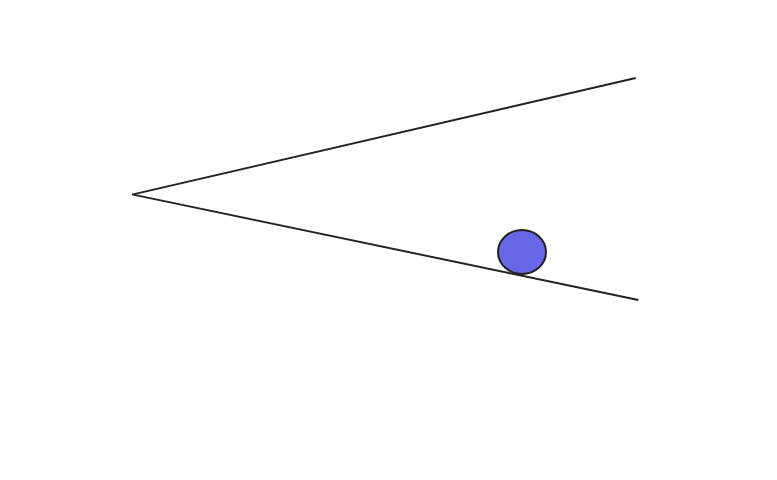
\includegraphics[width=200px]{images/BAD_CIRCLE.png}

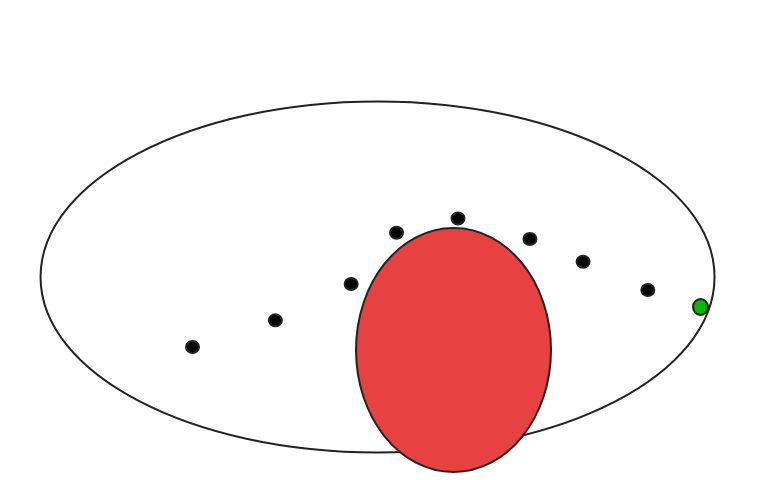
\includegraphics[width=200px]{images/infeasible_constraint.png}
\includegraphics[width=200px]{images/good_bad_geometry.png}







\section{Introduction}

Derivative free optimization (DFO) refers to mathematical programs involving functions for which derivative information is not explicitly available.
Such problems arise, for example, when the functions are evaluated by simulations or by laboratory experiments.
In such applications, function evaluations are expensive, so it is sensible to invest significant computational resources to minimize the number of function evaluations.

This work is aimed at developing algorithms to solve constrained optimization problems of the form 

\[ \begin{array}{ccl} \min_{x \in \domain} & f(x) \\
\mbox{subject to} & c_i(x) \le 0 & i \in \mathcal{I} \\
& c_i(x) = 0 & i \in \mathcal{E},
\end{array}
\]
where $\domain$ is a subset of $\real^n$, and $f$ and $c_i, i \in \mathcal{I} \cup \mathcal{E}$ are real-valued functions on $X$ with at least one of these functions being a {\em black-box} function, meaning that derivatives cannot be evaluated directly.  

In our work, we assume that all of the functions in the problem are black-box functions.
We consider two variations of this problem.
In the first variation, we assume that the constraints are fully quantifiable.


As in \cite{DUMMY:typesofconstraints}, this means that all of the functions can be evaluated at any point in $X$ and that the values returned for the constraint functions provide meaningful information about how close the point is to a constraint boundary.
In the second variation, we assume that the black-box functions return meaningful numerical values only when evaluated at feasible points. In this case, the constraints are called {\em partially quantifiable}.   


We are interested in developing {\em model-based} trust-region algorithms for solving these problems.
Model-based methods work by constructing model functions to approximate the black box functions at each iteration.
The model functions are determined by fitting previously evaluated function values on a set of sample points.
In trust-region methods, the model-functions are used to define a trust-region subproblem, whose solution determines the next iterate.
For example, the trust-region subproblem might have the form

\[ \begin{array}{ccl} \min_{\norm{s} \le \Delta}
 & m_{f}(x^k+s) \\
\mbox{subject to} & m_{c_i}(x^k+s) \le 0 & i \in \mathcal{I} \\
& m_{c_i}(x^k) = 0 & i \in \mathcal{E},
\end{array}
\]
where $m_{f}, m_{c_i}, i \in \mathcal{I} \union \mathcal{E}$ are the model functions, and $\Delta$ is the radius of the trust-region.
Conceptually, the model functions are ``trusted'' only within a distance $\Delta$ of the current iterate $x^k$; so the trust-region subproblem restricts the step $s$ to be no larger than $\Delta$.
To ensure that the model functions are good approximations of the true functions over the trust region, the sample points are typically chosen to lie within, or at least near, the trust-region.


An important consideration in fitting the model functions is the the ``geometry'' of the sample set.
This will be discussed in more detail in Section \ref{geometry}, but the key point is that the relative positions of the sample points within the trust region has a significant effect on the accuracy of the model functions over the trust region.
When the geometry of the sample set is poor, it is sometimes necessary to evaluate the functions at new points within the trust region to improve the geometry of the sample set.
A more detailed discussion can be found in \cite{doi:10.1080/10556780802409296}, but this step is required for convergence analysis although it may come at the expense of function evaluations.

In the case of partially quantifiable constraints, all of the sample points must lie within the feasible region.  This poses some interesting challenges for the geometry of the sample set.  As a first step toward developing an algorithm to solve such problems, we consider a simplified problem where all of the constraints are linear, but we impose the restriction that all sample points must lie within the feasible region.  This work is presented in Chapter \ref{feasiblemethod}

In the case of fully quantifiable constraints, there is no difficulty in using sample points outside of the feasible region.  
In Chapter \ref{chap:Filter}, we describe a Trust-Region SQP Filter method for solving this class of problems.

  
  
  
\section{Background}

\subsection{Strategy}
A reasonable approach to DFO is to modify classical algorithms that rely on derivatives by using the derivatives of the model functions whenever a derivative is needed in the algorithm.
However, the lack of explicit derivatives pose several challenges, which necessitate changes in the classical algorithms.
First, care must be taken to ensure that the model functions are sufficiently accurate approximations to the true functions.
This means that geometry of the sample points must be considered.
It also means that the trust-region radius must get arbitrarily small.

The transition to the derivative-free setting also provides some interesting research opportunities.
In particular, because function evaluations are so costly, there is potential for significant gains by considering more complex optimization paradigms.
For example, Sequential Quadratic Programming (SQP) methods use subproblems involving quadratic approximations of the objective function $f$ and linear approximations of the constraint functions.
In the derivative-free setting, it may be worthwhile to explore other variations of the classical algorithms.
For example, it might be worthwhile to construct quadratic models of the constraint functions, which might result in fewer iterations overall.

It might also be worthwhile to consider using different sample sets for fitting different functions.  

For example, the SQP trust-region filter method involves constructing a quadratic model of the objective function and linear models of the constraint functions.  But this raises an interesting question, since a good sample set for constructing a quadratic model may not be ideal for fitting the linear functions modeling the constraints.  

\subsection{Recent Work}


Within  \cite{DUMMY:intro_book} derivative-free methods are developed in detail.
This is the first text book devoted to derivative free optimization.
It contains a good explanation of ensuring geometry of the current set with poisedness for unconstrained problems and also covers other derivative-free methods including direct-search and line search.

A good review of derivative free algorithms and software libraries can be found in \cite{DUMMY:review}.
This compares several software libraries, and reviews the development of derivative free optimization since it started.
Another recent review can be found in \cite{DUMMY:review2}.





\paragraph{Applications}
A number of applications of derivative free optimization have risen recently including .
To reliability based optimization \cite{Gao2017}.
Larson co-authored \cite{1742-6596-874-1-012062}.
To parallel computing \cite{Cheng2017}
To circuitry arrangements \cite{PLOSKAS201816}
\cite{KS2018}


\paragraph{Complexity Analysis}

A derivation is found in \cite{doi:10.1137/151005683} which shows that a bound of $O(\epsilon^{-2})$ and $O(n^2\epsilon^{-2})$ function evaluations.
Using cubic over estimation using finite differences $O(\epsilon^{-1.5})$.
 function evalutaions.

 
\cite{doi:10.1093/imanum/drx043}


\begin{verbatim}
https://arxiv.org/abs/1710.11005
\end{verbatim}
Replaces quadratic models with residual linear models


\paragraph{Related Algorithms}

\cite{doi:10.1080/10556788.2015.1026968}

\cite{Tröltzsch2016}
\cite{infeasiblestarting}
\cite{Gao2018}




%\section{Subproblems}
%\cite{doi:10.1080/10556780802409296}
%\cite{DBLP:journals/ol/KamandiAA17}
%\cite{Verdério2017}
%\cite{Powell2015}
%\cite{AMAIOUA201813}
%\cite{Kamandi2017}




%Within \cite{DUMMY:linesearch_global} and \cite{DUMMY:linesearch_local} Biegler uses a filter method to ensure global convergence within a line search framework.
%Could talk about filter methods



\cite{Conejo:2013:GCT:2620806.2621814}
\cite{doi:10.1137/151005683}
\cite{Audet2016APB}
\cite{Tröltzsch2016}
\cite{doi:10.1080/02331934.2016.1263629}
\cite{infeasiblestarting}
\cite{doi:10.1080/10556780802409296}
\cite{doi:10.1080/10556788.2015.1026968}
\cite{doi:10.1093/imanum/drx043}
\cite{Beyhaghi2017}
\cite{Golovin:2017:GVS:3097983.3098043}
\cite{DBLP:journals/ol/KamandiAA17}
\cite{1742-6596-874-1-012062}
\cite{KS2018}
\cite{8247938} 
\cite{doi:10.1002/aic.16364}
\cite{AuHa2017}
\cite{Verdério2017}
\cite{Gao2017}
\cite{Cheng2017}
\cite{Martínez2013}
\cite{AMAIOUA201813}
\cite{Amaran2014}
\cite{Costa2014RBFOptA}
\cite{doi:10.1137/15M1031679}
\cite{Gao2018}
\cite{PLOSKAS201816}
\cite{doi:10.1137/1.9781611974683.ch37}
\cite{Powell2015}
\cite{Kamandi2017}
\cite{Kieslich2018}
\cite{DUMMY:Biegler}
\cite{DUMMY:Fletcher}
\cite{DUMMY:Brekelman}
\cite{DUMMY:CombineTrustAndLine}
\cite{DUMMY:linesearch_global}
\cite{DUMMY:linesearch_local}
\cite{DUMMY:intro_book}
\cite{DUMMY:trust_funnel_dfo}
\cite{DUMMY:original_filter}
\cite{DUMMY:sqp_filter}
\cite{DUMMY:Colson2004}
\cite{DUMMY:SQPFilter}
\cite{DUMMY:Rios2013}
\cite{DUMMY:PowellRadialBasis}
\cite{DUMMY:leastsquares}
\cite{DUMMY:typesofconstraints}
\cite{DUMMY:FasanoLLR14}
\cite{DUMMY:filterpattern}
\cite{DUMMY:activeset1}
\cite{DUMMY:LiuzziLS10}
\cite{DUMMY:augmented}






\subsubsection{Model-based, Trust Region Methods}
We will be modifying the following classical algorithm described at a high level here.
A set of poised points are chosen for some radius $\Delta_k>0$ about the current iterate.
The objective and constraints are then evaluated at these points to construct a model function as a linear combination of some set of basis functions.
Next, the model is minimized over this trust region and the argument minimum becomes the trial point.
The objective is evaluated at the trial point and a measure of reduction $\rho$ is computed.
If $\rho$ implies that sufficient reduction has been made and that the model approximates the function well, the trial point is accepted as the new iterate.
Otherwise, the trust region is reduced to increase model accuracy.


For unconstrained optimization, the algorithmic framework can be described with these steps:

\begin{enumerate}
	\item Create a model function $m_k(x)$.
	\begin {itemize}
		\item In classical trust region methods, the following quadratic model function is used:
		\[
		m_k(x) = f(x^{(k)}) + \nabla f(x^{(k)})^T (x-x^{(k)}) + \frac 1 2 (x-x^{(k)})^T\nabla^2f(x^{(k)})(x-x^{(k)})
		\]
	\end{itemize}
	\begin{itemize}
		\item $\nabla f(x^{(k)})$ and $\nabla^2 f(x^{(k)})$ must be approximated
		\item Geometric properties of the sample set that must be satisfied
	\end{itemize}
	
	\item If $\nabla m_k(x) < \tau$ stop, where $\tau$ is some tolerance
	
	\item Solve the Trust region subproblem: $s^{(k)} = \argmin_{s\in B(x^{(k)};\Delta_k)} m_k(x^{(k)} + s)$
	\begin {itemize}
		\item $B(x^{(k)};\Delta_k) = \{ x \in \mathbb{R}^n : \| x - x^{(k)} \le \Delta_k \}$ 
		is the ball of radius $\Delta_k$ centered at $x^{(k)}$
	\end{itemize}
	
	\item Test for improvement
	\begin{itemize}
		\item Compute
\begin{equation}
\label{rho}
\rho_k = \frac{f(x^{(k)}) - f(x^{(k)}+s^{(k)})}{m_k(x^{(k)}) - m_k(x^{(k)}+s^{(k)})}
\end{equation}
which measures the actual improvement over predicted improvement
		\item If $\rho$ is small, $x^{(k+1)}=x^{(k)}$ (reject) and decrease radius
		\item If $\rho$ is intermediate, $x^{(k+1)}=x^{(k)}+s^{(k)}$ (accept) and decrease radius
		\item If $\rho$ is large, $x^{(k+1)}=x^{(k)}+s^{(k)}$ (accept) and either increase the radius or decrease if $\nabla m_k(x_k)$ is small
	\end{itemize}
	
	\item Go to step 1
\end{enumerate}

Our goal is generalize this framework to handle constraints, where we must reduce constraint violation while ensuring the accuracy of the models of the constraints.

  
%\subsection{Constrained DFO}
%Derivative free optimization problems can be broken into several categories based on the form of functions within the program.
%Several of these categories are described nicely in \cite{DUMMY:typesofconstraints}.
%For example, a typical constrained program within DFO is given by:
%\[ \begin{array}{ccl} \min & f(x) \\
%\mbox{subject to} & c_i(x) \le 0 & i \in \mathcal{I} \\
%& c_i(x) = 0 & i \in \mathcal{E}
%\end{array}
%\]
%where at least one of the functions $f, c_i, i \in \mathcal{I} \cup \mathcal{E}$ is a black box function,
%meaning that we have no information about its derivatives.
% If $c(x, S(x)) = c(x)$, then 

%A well studied case is when the derivatives of $c$ are known, so the objective is the only derivative free function.
%For example, there several libraries exist for Box Constrained DFO (BCDFO) where the constraints take the form $b_{L} \le x \le b_{U}$ for some $b_{L} < b_{U}$.
%However, the problem becomes more difficult in our case where no derivative information of $c$ or $f$ is known.

\subsubsection{Interpolation/regression methods}

Within interpolation model-based methods, we construct our model by regressing basis functions onto a set of sampled points.
For example, given a function $f(x) : \mathbb R^n \to \mathbb R$ we can use a set of basis functions $\phi_i : \mathbb R^n \to \mathbb R \quad \forall 1 \le i \le d_1$ to construct a model function $m(x) = \sum_{i=1}^{d_1} \lambda_i \phi_i(x)$ approximating $f(x)$ by selecting appropriate $\lambda_i \in \mathbb R$.
This is done by choosing a set of sample points
$Y = \{y^1, y^2, \ldots, y^{d_2}\}$,
evaluating $f = (f_1 = f(y^1), f_2 = f(y^2), \ldots, f_d = f(y^{d_2}))^T$
and forcing model agreement with the original function $f(x)$ by ensuring

\begin{equation}
\label{reg}
\begin{bmatrix}
    \phi_1(y^1)      & \phi_2(y^1)       & \ldots & \phi_{d_1}(y^1)      \\
    \phi_1(y^2)      & \phi_2(y^2)       & \dots  & \phi_{d_1}(y^2)      \\
                     &                   & \vdots &                      \\
    \phi_1(y^{d_2})  & \phi_2(y^{d_2})   & \ldots & \phi_{d_1}(y^{d_2})
\end{bmatrix}
\begin{bmatrix}
    \lambda_1      \\
    \lambda_2      \\
    \vdots         \\            
    \lambda_{d_1}
\end{bmatrix}
\approx
\begin{bmatrix}
    f_1      \\
    f_2      \\
    \vdots         \\            
    f_{d_2}
\end{bmatrix}.
\end{equation}

When $d_1 = d_2$ this is called interpolation and equality is desired within \ref{reg}.
% It could be important to discusss this, because we may use different orders for the constraints than the objective.
%When $d_1 < d_2$ this is called underdetermined interpolation, 
%This can be handled by requesting and a minimum norm solution.
%Finally, when $d_1 > d_2$ this is called regression and only a least squares solution can be requested.
Note that in practice, the set $Y$ is shifted and scaled.

\paragraph{Sampling issues}

These methods can have issues with poor sampling choices.
Two important aspects of the sample points are their geometry and proximity.

\subparagraph{Geometry}
\label{geometry}

For geometry, regression based methods require that the set the function is evaluated at must be $\Lambda$-poised for a fixed constant $\Lambda$.
If the set is $\Lambda$-poised for a certain trust region radius, then the maximum absolute value of any Lagrange polynomial over the trust region is one.
This ensures that the Vandermonde matrix used to find the coefficients used to express the model function in terms of a basis of Lagrange polynomials is well conditioned.
Although we do not go into the details here, problems become apparent when comparing the Lagrange polynomials associated with a poised set with those of an ill poised set.

In the following image, a set of quadratic polynomials used to interpolate the function $5 + x + y + (x + y) ^ 2 - \alpha y ^ 4$.
However, the sample points are chosen to be nearly colinear.

\includegraphics[width=200px]{images/bad_geometry.png}



\subparagraph{Proximity}

Proximity refers to the trust region radius.
The trust region must go to zero if we are to be sure that we have reached a critical point.
In general, the smaller the trust region, the closer to linear or quadratic the original function will look.
This is because the model's error term given by Taylor's expansion is proportional to the trust region radius.


%\paragraph{Types of constraints}
%%Regression based methods work by evaluating model functions on a set of sample points to construct local models of the functions.
%%This atleast allows the algorithm to minimize these easier model functions over a trust region, rather than working with the original function.

%One distinction important to the choice of sample points is fully quantifiable constraints versus partially-quantifiable constraints.
%If the constraints are fully quantifiable, they can be evaluated anywhere and present no restriction to the sample points.
%However, partially-quantifiable constraints only produce meaningful values within the feasible region.

%If the constraints are fully-quantifiable, a trust-region filter method can be used.
%We describe this approach in \ref{}.
%When the constraints are partially-quantifiable, the goal is to modify the trust region to avoid evaluating the simulation function outside of the feasible region.
%This is described in \ref{}.
%
%For the first step towards developing this algorithm, we develop develop an algorithm that uses linear constraints to model a linearly constrained region.
%This is described in \ref{feasiblemethod}


%\color{red} Within noisy optimization, this gives rise to several more problems. If you think there is something else about proximity that I should mention, please let me know. \color{black}

\subsection{Setting}

%We will be considering problems of the form


%\begin{center}
%\begin{align}
%\label{problem}
%\min_x & \quad f(x) \\
%  c_i(x) \le 0   & \quad \forall i \in \mathcal {I} \nonumber \\
%  c_i(x)  = 0    & \quad \forall i \in \mathcal {E} \nonumber
%\end{align}
%\end{center}
%where $f : \mathbb R^n \to \mathbb R$, and each $c_i : \mathbb{R} \to \mathbb{R}$.
It will be convenient to write
$c_{\mathcal {I}}(x) = (c_1(x), c_2(x), \ldots, c_{|\mathcal{I}|})^T$,
$c_{\mathcal {E}}(x) = (c_{|\mathcal{I}|+1}(x), c_{|\mathcal{I}|+2}(x), \ldots, c_{|\mathcal{I}| + |\mathcal{E}|})^T$ and
$c(x) = (c_{\mathcal{I}}^T(x), c_{\mathcal{E}}^T(x))^T$.


At an iteration $k$, we first construct a model function $m_f^k(x)$ that we use to approximate the first and second derivatives of $f(x)$.
We also construct $m_{\mathcal{I}}^k(x)$ and $m_{\mathcal{E}}^k(x)$ to approximate the first derivatives of $c(x)$.
Namely, at an iterate $x^k$, we let $f^k = f(x^k)$, $g^k = \nabla m_f^k(x^k)$. %be the gradient of the objective's model at $x^k$.
We also define the $c_{{\mathcal{I}}}^k = c^k_{\mathcal{I}}(x^k)$, 
$A_{{\mathcal{I}}}^k = \nabla m_{\mathcal{I}}^k(x^k)$,
$c_{{\mathcal{E}}}^k = c_{\mathcal{E}}(x^k)$, and
$A_{{\mathcal{E}}}^k = \nabla m_{\mathcal{E}}^k(x^k)$.

It will also be convenient to let $\mathcal{F}^k = \{ x \in \mathbb R^n | c_i(x) \le 0 \forall i \in \mathcal{I} \wedge c_i(x) = 0 \forall i \in \mathcal{E}\}$ be the feasible region.

We work within a trust region, sequential quadratic programming framework with interpolating model functions.
%For our algorithm, we assume that all functions are derivative-free: all functions are evaluated by a single call to a black box function:
%$S(x) = (f(x), c_{\mathcal {I}}(x)^T, c_{\mathcal {E}}(x)^T)^T$.

%\color{blue}
%We also assume that we are not able to evaluate points outside the feasible region.
%This introduces a new type of constraint: it is not quite a hidden constraint because we do observe function values within the feasible region.
%However, it does implies similar difficulty to construct the model function near the boundary of the feasible region because we have limited sampling ability.
%\color{black}

We first compute an interpolation set poised for regressing a set of model functions, which we choose to be quadratic functions.
Although we have enough sample points to construct a quadratic model of the constraints, we only construct linear models to avoid the complexity of Quadratically Constrained Quadratic Programming which is NP-hard.

\subsubsection{Model functions}


%We will also need to compute the Hessian of the Lagrangian for \ref{problem}.
%The Lagrangian is defined as 
% $L(x, \mu, \lambda) =
% f(x)  
% + \sum_{i \in {\mathcal{I}}} \mu_i     c_i(x)
% + \sum_{i \in {\mathcal{E}}} \lambda_i c_i(x)$.
%To compute its second derivative, we let $A^k$ and $c^k$ contain $A_{\mathcal{E}}^k$ and $c_{\mathcal{E}}^k$ as well as any rows of $A_{{\mathcal{I}}}^k$ and %$c_{\mathcal{E}}^k$ corresponding
%to active constraints at $x^k$.
%The set of active constraints $\mathcal A \subseteq \mathcal I \cup \mathcal E$ includes $\mathcal E$ and any $i \in \mathcal I$ for which $c_i(x^k) \ge 0$.
%We then solve the system
%\begin{align*}
%\nabla^2m_k(x_k) & d + {A^k}^T\lambda & = g^k \\
%A^k              & d                & = c^k
%\end{align*}
%for $\lambda$ and compute
%\[
%H^k = \nabla^2 m_k(x^k) 
%+ \sum_{i \in \mathcal E} \lambda_i \nabla^2 m_{g,i}^k(x^k) 
%+ \sum_{i \in \mathcal A \backslash \mathcal E} \lambda_i \nabla^2 m_{h,i}^k(x^k).
%\]

%With these definitions, we define the quadratic subproblem as

%\begin{align*}
%\argmin_s  f(x^k+s) = f^k + (g^k)^Ts + \frac 1 2 (s^k)^T H^ks^k  &\\
%     c_{{\mathcal{I}}}^k + A_{{\mathcal{I}}}^ks       &\le \; 0  \\
%s.t. \hspace{1cm} c_{{\mathcal{E}}}^k + A_{{\mathcal{E}}}^ks           &=\; 0 \\
%     \| s \|                      &\le \; \Delta_k.
%\end{align*}



\subsubsection{Criticality Measure}

In order to construct stopping criteria, we introduce a criticality measure $\chi$ which goes to zero as the iterates approach a first order critical point.
Once this has reached small enough threshold, and the trust region is small enough, we can terminate the algorithm.
For now, our algorithm is designed to work with convex constraints, so emply a classic criticallity measure of

\[
\chi(x) = \|x - Proj_{\domain}(x - \nabla m_f(x))\|
\]

This can be computed as 
\[
\label{critical}

\chi_k = \chi(x_k) = \| \argmin s \|
\]



%That is, if $x^{\star}$ is a first order critical point satisfying

%\begin{align*}
%\nabla f(x^{\star}) + \sum_{i\in\mathcal I} \lambda_i \nabla c_i(x^{\star}) + \sum_{i\in \mathcal E} \mu_i \nabla c_i(x^{\star})  = 0 \\
%c(x^{\star})_i \mu_i = 0 & \quad \forall i\in\mathcal I \\
%c(x^{\star}) \le 0 & \quad \forall i\in\mathcal I\\
%c(x^{\star}) = 0 & \quad \forall i\in\mathcal E
%\end{align*}
%for some $\lambda_i \in \mathbb R$, and $\mu_i \ge 0$, then we need $\lim_{x\to x^{\star}} \chi(x) = 0$.

%This suggests the following definition:
%\begin{align}
%\label{critical}
%\chi & = & |\min_t \langle g_k + H_kn_k, t\rangle| \\
%& A_{\mathcal {E}}t &=& \; 0 \\
%& c_{\mathcal {I}} + A_{\mathcal {I}}t &\le& \; 0 \\
%& \| t \| &\le& \; 1
%\end{align}

%Notice that this must be computed after the normal step $n^k$ has been computed.

%\color{red}
%\subsubsection{Sufficient reduction of model}
%It is not enough to simply ask for decrease in the objective every iteration.
%We also require \emph{sufficient} reduction, so that any accumulation point of the sequences of iterates is feasible.
%o this end, we introduce constants $0 < \kappa_{\theta} < 1$ and $\psi > \frac{1}{1+\mu}$ and require

%\begin{equation}
%\label{predicted_decrease}
%m_k(x_k) - m_k(x_k+s_k) \ge \kappa_{\theta} \theta_k^{\psi}.
%\end{equation}
%\color{black}

%\color{red}
%Although this only references the model functions, we ensure accuracy by computing $\rho$.
%\color{black}

%\subsubsection{Compatibility}

%\newpage
%\subsection{The Algorithm}

%With these tools, we can now describe the algorithm.
%The overall steps are as follows:

%\underline{\hspace{20cm}}
%\FloatBarrier
%\begin{enumerate}
%\item \textbf{Initialize} each constant introduced so far

%\item \textbf{Compute model functions} $m_f$, $m_g$, $m_h$, the active constraints $\mathcal A$, and the Hessian of the Lagrangian $H_k$

%\item \textbf{Compute the normal step} $n_k$ according to \ref{normal}

%If the feasible region of \ref{normal} is empty or \ref{compat} is not satisfied, then 
%\begin{itemize}
%\item Add $(\theta_k, f_k)$ to the filter
%\item Call the feasibility restoration routine
%\item Increment $k$
%\item Go to step 2
%\end{itemize}

%\item \textbf{Compute criticality measure} $\chi$ from \ref{critical}
%\begin{itemize}
%\item If $\chi$ is small, but the trust region radius is larger than the tolerance, then decrease the trust region, increment $k$ and return to step 2
%\item Otherwise, if $\chi$ and the trust region radius is smaller than the tolerance, return success
%\item If $\chi$ is zero, then return success
%\end{itemize}


%\item \textbf{Compute tangential step} $t_k$ according to \ref{tangent}

%Define $s_k = n_k + t_k$.

%\item Check for \textbf{sufficient reduction} in the model function

%If \ref{predicted_decrease} is satisfied
%\begin{itemize}
%\item Add $(\theta_k, f_k)$ to the filter
%\item Increment $k$
%item Go to step 2
%\end{itemize}

%\item \textbf{Evaluate} the function and constraints at the trial point $x_k + s_k$

%If the new point is not acceptable to the filter according to either \ref{acceptable1} or \ref{acceptable2}, then
%\begin{itemize}
%\item Add $(\theta_k, f_k)$ to the filter
%\item Increment $k$
%\item Go to step 2
%\end{itemize}

%\item \textbf{Compute $\rho$} according to \ref{rho}
%\begin{itemize}
%\item If $\rho \le \gamma_1$ is small, then decrease the trust region radius and go to step 2
%\item If $\gamma_1 < \rho \le \gamma_2$ is intermediate, then accept the trial point $x_{k+1} = x_{k} + s_k$.
%\item If $\rho > \gamma_2$, and $\chi$ is small, then decrease the trust region radius.
%\item If $\rho > \gamma_2$ is large, and $\chi$ is large, then increase the trust region radius.
%\end{itemize}

%\item increment $k$ and go to step 2
%\end{enumerate}
%\FloatBarrier

%\underline{\hspace{20cm}}



\section{Algorithms}
\label{feasiblemethod}


\subsection{Algorithm Template}



$k \leftarrow k + 1$


\begin{enumerate}
    \item Initialize $k=0$, $0<\gamma_1<\gamma_2<1$,$\tau_{\chi}>0$,$\tau_{\Delta}>0$, $\Delta_0 > 0$, $x_0$ a feaisble starting point, $0<\omega_{\text{dec}} < 1 \le \omega_{\text{inc}}$, $\gamma_{\Delta}$
    \item Compute the inner trust region.
    \begin{itemize}
        \item This may mean maximizing an ellipse as in \ref{ellipse_optimization}
    \end{itemize}
	\item Ensure poisedness, and create the model functions ${m_f}_k(x)$, ${c_i}_k(x), i \in \mathcal I \cup \mathcal E$ as described in \ref{reg}
	\item Compute critically measure $\chi_k = \chi(x_k)$ as described in \ref{critical}
    \begin{itemize}
        \item If $\chi_k < \tau_{\chi}$ and $\Delta_k <= \tau_{\Delta}$, return as converged
        \item If $\chi_k < \tau_{\chi}$ and $\Delta_k > \tau_{\Delta}$, then $\Delta_{k+1} \leftarrow \omega_{\text{dec}} \Delta_k$, $k \leftarrow k + 1$
    \end{itemize}
	
	\item Solve the Trust region subproblem: $s^{(k)} = \argmin_{s\in B(x^{(k)};\Delta_k)} m_k(x^{(k)} + s)$
	\begin {itemize}
	\end{itemize}
	
	\item Test for improvement
	\begin{itemize}
		\item Compute $\rho_k = \frac{f(x^{(k)}) - f(x^{(k)}+s^{(k)})}{m_k(x^{(k)}) - m_k(x^{(k)}+s^{(k)})}$
    \begin{equation}
    \item \end{equation}
		\item If $\rho < \gamma_1$, then $x^{(k+1)}=x^{(k)}$ (reject) $\Delta_{k+1} \leftarrow \omega_{\text{dec}} \Delta_k$
		\item If $\gamma_1 \le \rho \le \gamma_2$, then $x^{(k+1)}=x^{(k)}+s^{(k)}$ (accept) and $\Delta_{k+1} \leftarrow \omega_{\text{dec}} \Delta_k$
		\item If $\rho > \gamma_2$, then $x^{(k+1)}=x^{(k)}+s^{(k)}$ (accept)
		\begin{itemize}
            \item If $\|x^{(k)} - s^{(k)} \| < \gamma_{\Delta} \Delta_k$ then $\Delta_{k+1} \leftarrow \omega_{\text{dec}} \Delta_k$
            \item else $\Delta_{k+1} \leftarrow \omega_{\text{inc}} \Delta_k$
		\end{itemize}
	\end{itemize}
    $k \leftarrow k + 1$
	
	
	
	\item Go to step 2
\end{enumerate}






\section{Simple approach}
One simple approach to handling hidden constraints is to simply avoid letting points fall outside the feasible region.

Within this model, we maintain the same policies for updating the trust region radius.
However, within the LU factorization algorithm to select new points, we add to the trust region subproblem that the new points must also lie within the current model of the trust region.

This can happen when the feasible region intersect the trust region is small compared to the trust region.
As the number of dimensions grows, this can become worse.

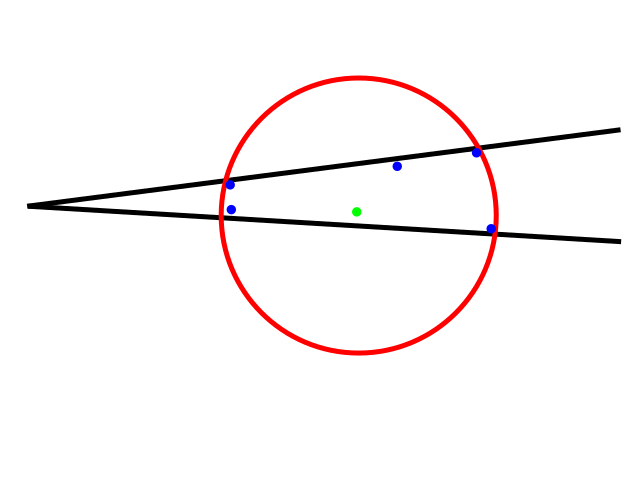
\includegraphics[scale=0.4]{bad_lambda.png}


\includegraphics[width=200px]{images/good_bad_geometry.png}

\section{Bumping $\xi$}


Within the classical algorithm, we used $\xi$ as a lower bound of the pivot values of the Vandermode matrix.
When requiring points to live within the trust region intersect the feasible region, it can happen that even after replacing a point, we still have not satisfied this bound.
One way to handle this is to simply allow $\xi$ to decrease until a threshold is reached.
(The threshold is for maintaining a fixed lambda.)


    
\section{Ellipse}


We decided to keep the trust region entirely within the feasible region because of the high lambda when only requiring the points to lie in the feasible region.
In order to deal with the numerical problems from having a circular trust region, we can map the feasible region back to a circle.
More specifically, at iteration $k$, we select an ellipse center $\mu^k$, a scaling factor $\pi^k$ and positive definite matrix $Q^k$ to define and ellipse
$E_k = \{x \in \mathbb R^n \| \pi^k - \frac 1 2 (x - \mu^{k})^TQ^{k}(x - \mu^{k}) \ge 0 \}$.
We then map this back to the origin with the affine transformation $T^k : \mathbb R^n \to R$ $T^k(x) = \frac {\sqrt{2}}{\pi^k} L^k(x-\mu^k)$ where $L = cholesky(Q)$.
This will allow us to construct a lambda poised set within narrow trust regions.

There are a number of issues to be solved to define this ellipse:
\begin{itemize}
\item How do we ensure that $x^k \in E^k$?
\item How do we choose the center of the ellipse $\mu^k$?
\item Is $E_k \subset F_k$?
\end{itemize}

We have tried a couple of ways of ensuring the current iterate is within the trust region, $x^k \in E^k$.
If we do not include the current iterate \color{red} within the interior \color{black}, we likely lose sufficient reduction.
This can be done by either expanding the radius of the ellipse, or by including the original point as a constraint for the ellipse problem.

% Insert images here.

In order to include the original point as a constraint, we simply add the following constraint to the definition of the ellipse:
$$ \pi^k - \frac 1 2 (x^k - \mu^{k})^TQ^{k}(x^k - \mu^{k}) \ge 0. $$
However, the optimization problem we construct to find $Q^k$ solves for ${Q^k}^{-1}$, so that adding this constraint is a constraint on the inverse of $Q^k$.



%\begin{center}
%\begin{align}
%\label{problem}
%\min_x & \quad m_f(x) \\
%  m_{c_i}(x) \le 0   & \quad \forall i \in \mathcal {I} \nonumber \\
%  m_{c_i}(x)  = 0    & \quad \forall i \in \mathcal {E} \nonumber \\
%  \bar{x}^T Q^k \bar{x} \le s^k
%\end{align}
%\end{center}


The alternative is to scale $Q$ by a constant.
To do this, we use the scaling factor $\pi^k$ by defining it to be

$$\pi^k = \max \{1, \frac 1 {2} (x^{k} - \mu^{k})^T Q^k (x^{k} - \mu^{k})^T \}$$

and let the ellipse be:
$$\{x \in \mathbb | 1 - \frac 1 {2\pi^k} (x - \mu^{k})^T Q (x - \mu^{k}) \ge 0\} $$
However, this means that we do not ensure $E_k \subset F_k$ so that the trust region subproblem must contain constraints for both the ellipse and the feasible region.


The are some concerns we have to consider while defining the ellipse.
One major concern is that we can accidently define the ellise in a way that forces the trust region away from the desired drection.
Also, unless we include points outside the ellipse, we cannot find a second order solution because the ellipse can only be tangent to the constraint.
We also want consecutive ellipse to share volume, in order to avoid evaluating as many points as possible.
(So far, we have been re-evaluating the set of trial points each iteration.)
Finally, we have the problem of computing the ellipse once given a suitable definition.


\subsection{Finding the maximal $E_k$ given $\mu^k$}

\label{ellipse_optimization}

Within this paper, we first solve the problem of finding the maximal ellipse given the center, and then perform a simple search over different centers of the ellipse.
Because of this, we will first show how to find an ellipse with maximal volume given a fixed center.
For now, we also let $s^k = 1$.

Given a polyhedron $P$ defined by an $m \times n$ matrix $A$,
\[
P = \{ x \; | \;  Ax \le b \},
\]
and we wish to find the largest ellipse $E \subset P$ centered at a point $\mu^{k}$ within this polyhedron.

We can shift the polyhedron by letting $\bar{b} = b - A\mu^{k}$ and letting $x \to x - \mu^{k}$ so that the polyhedron becomes
\[
P = \{ x \; | \;  Ax \le \bar{b} \}
\]
The ellipse can then be centered at zero, and defined by a positive semi-definite matrix $Q \succeq 0$:
\[
E = \{ d \; | \; \frac 1 2 d^T Q d \le 1 \}.
\]
where $Q = Q^T$.
We can define the auxiliary function 
\[
f(x) = \frac 1 2 x^T Q x
\]
so that this becomes
\[
E = \{ d \; | \; f(d) \le 1 \}.
\]


At the locations where the ellipse intersects the polyhedra with minimum value of $f$, the gradients of $f$ must be orthogonal to the faces.
Each face is defined by at least one $A_i x \le \bar{b}_i$ where $A_i$ is the $i$th row of $A$ for $1\le i \le m$.
This implies that if $d^{(i)}$ is such a point, then
\[
\nabla f(d^{(i)}) = \lambda_i A_i \quad \forall 1\le i\le m
\]
for some $\lambda_i$.
This means
\[
Q d^{(i)} = \lambda_i A_i \quad \forall 1\le i\le m
\]
\[
d^{(i)} = \lambda_i Q^{-1}A_i \quad \forall 1\le i\le m
\]
We also know that 
\[
A_i^T d^{(i)} = \bar{b} \quad \forall 1\le i\le m
\]
\[
A_i^T \lambda_i Q^{-1}A_i = \bar{b} \quad \forall 1\le i\le m
\]
\[
\lambda_i = \frac {\bar{b}}{A_i^T  Q^{-1}A_i} \quad \forall 1\le i\le m
\]
so that 
\[
d^{(i)} = \lambda_i Q^{-1}A_i \forall 1\le i\le m
\]
\[
d^{(i)} = \frac {\bar{b}}{A_i^T  Q^{-1}A_i}  Q^{-1}A_i \quad \forall 1\le i\le m.
\]

Finally, we need that for each $i$, $f(d^{(i)}) \le 1$:
\[
\frac 1 2 (d^{(i)})^{T} Q d^{(i)} \le 1
\]
\[
\frac 1 2 (\frac {\bar{b}}{A_i^T  Q^{-1}A_i}  Q^{-1}A_i)^{T} Q \frac {\bar{b}}{A_i^T  Q^{-1}A_i}  Q^{-1}A_i \le 1
\]
\[
\frac 1 2 \frac {1}{A_i^T  Q^{-1}A_i}  \bar{b}^T A_i^T Q^{-1} Q \frac {\bar{b}}{A_i^T  Q^{-1}A_i}  Q^{-1}A_i \le 1
\]
\[
\frac 1 2 \frac {1}{A_i^T  Q^{-1}A_i}  \bar{b}^T \frac {\bar{b}}{A_i^T  Q^{-1}A_i}  A_i^T Q^{-1}A_i \le 1
\]
\[
\frac 1 2 \bar{b}^T \frac {\bar{b}}{A_i^T  Q^{-1}A_i} \le 1
\]
\[
\frac 1 2 \bar{b}^T \bar{b}\le A_i^T  Q^{-1}A_i
\]
\[
A_i^T  Q^{-1}A_i \ge \frac 1 2 \bar{b}^T \bar{b}
\]

Thus, the maximal ellipse is defined by

\[
\sup_{Q \succeq 0} \det(Q^{-1})
\]
\[
s.t. \quad A_i^T Q^{-1} A_i \ge \frac 1 2 \bar{b}^T\bar{b}
\]


This problem includes a maximization of a determinant.
In order to ensure that the trust region goes to zero, we must also ensure that the maximum eigenvalue of the matrix is bounded.
Thus, for some bound $M^k$ we define $Q^k$ as

\begin{center}
\begin{align}
\label{ellipse_1}
Q^k = V(\mu_k) = \sup_{Q \succeq 0} & \det(Q^{-1}) & \\
  & {A^k}_i^T Q^{-1} {A^k}_i \ge \frac 1 2 (b^k - A^k\mu^{k})^T(b^k - A^k \mu^{k}) & \\
  & eig(Q)_i \le M^k & \forall i \in \mathcal I \cup \mathcal E \\
  & \pi^k - \frac 1 2 (x^k - \mu^{k})^TQ^{k}(x^k - \mu^{k}) \ge 0
\end{align}
\end{center}

if we wish to include the original point explicitly.
This gives rise to the trust region sub problem of

$$\{x \in \mathbb | 1 - \frac 1 {2s^k} (x - \mu^{k})^T Q (x - \mu^{k}) \ge 0\} $$
$$s^k = \max \{1, \frac 1 {2} (x^{k} - \mu^{k})^T Q^k (x^{k} - \mu^{k})^T \}$$






\subsection{Stationary center}
The simplest approach is to not change the center of the ellipse, but instead let $\mu^k = x^k$.
In the example below, we begin with a trust region that must be very small to lie within the feasible region, and note that if we even keep the same center, we are still able to search towards the vertex of the feasible region.
After solving the trust region subproblem in the first image, the iterate is near a constraint within the next iteration.
However, the ellipse elongates along an axis parallel to this constraint.

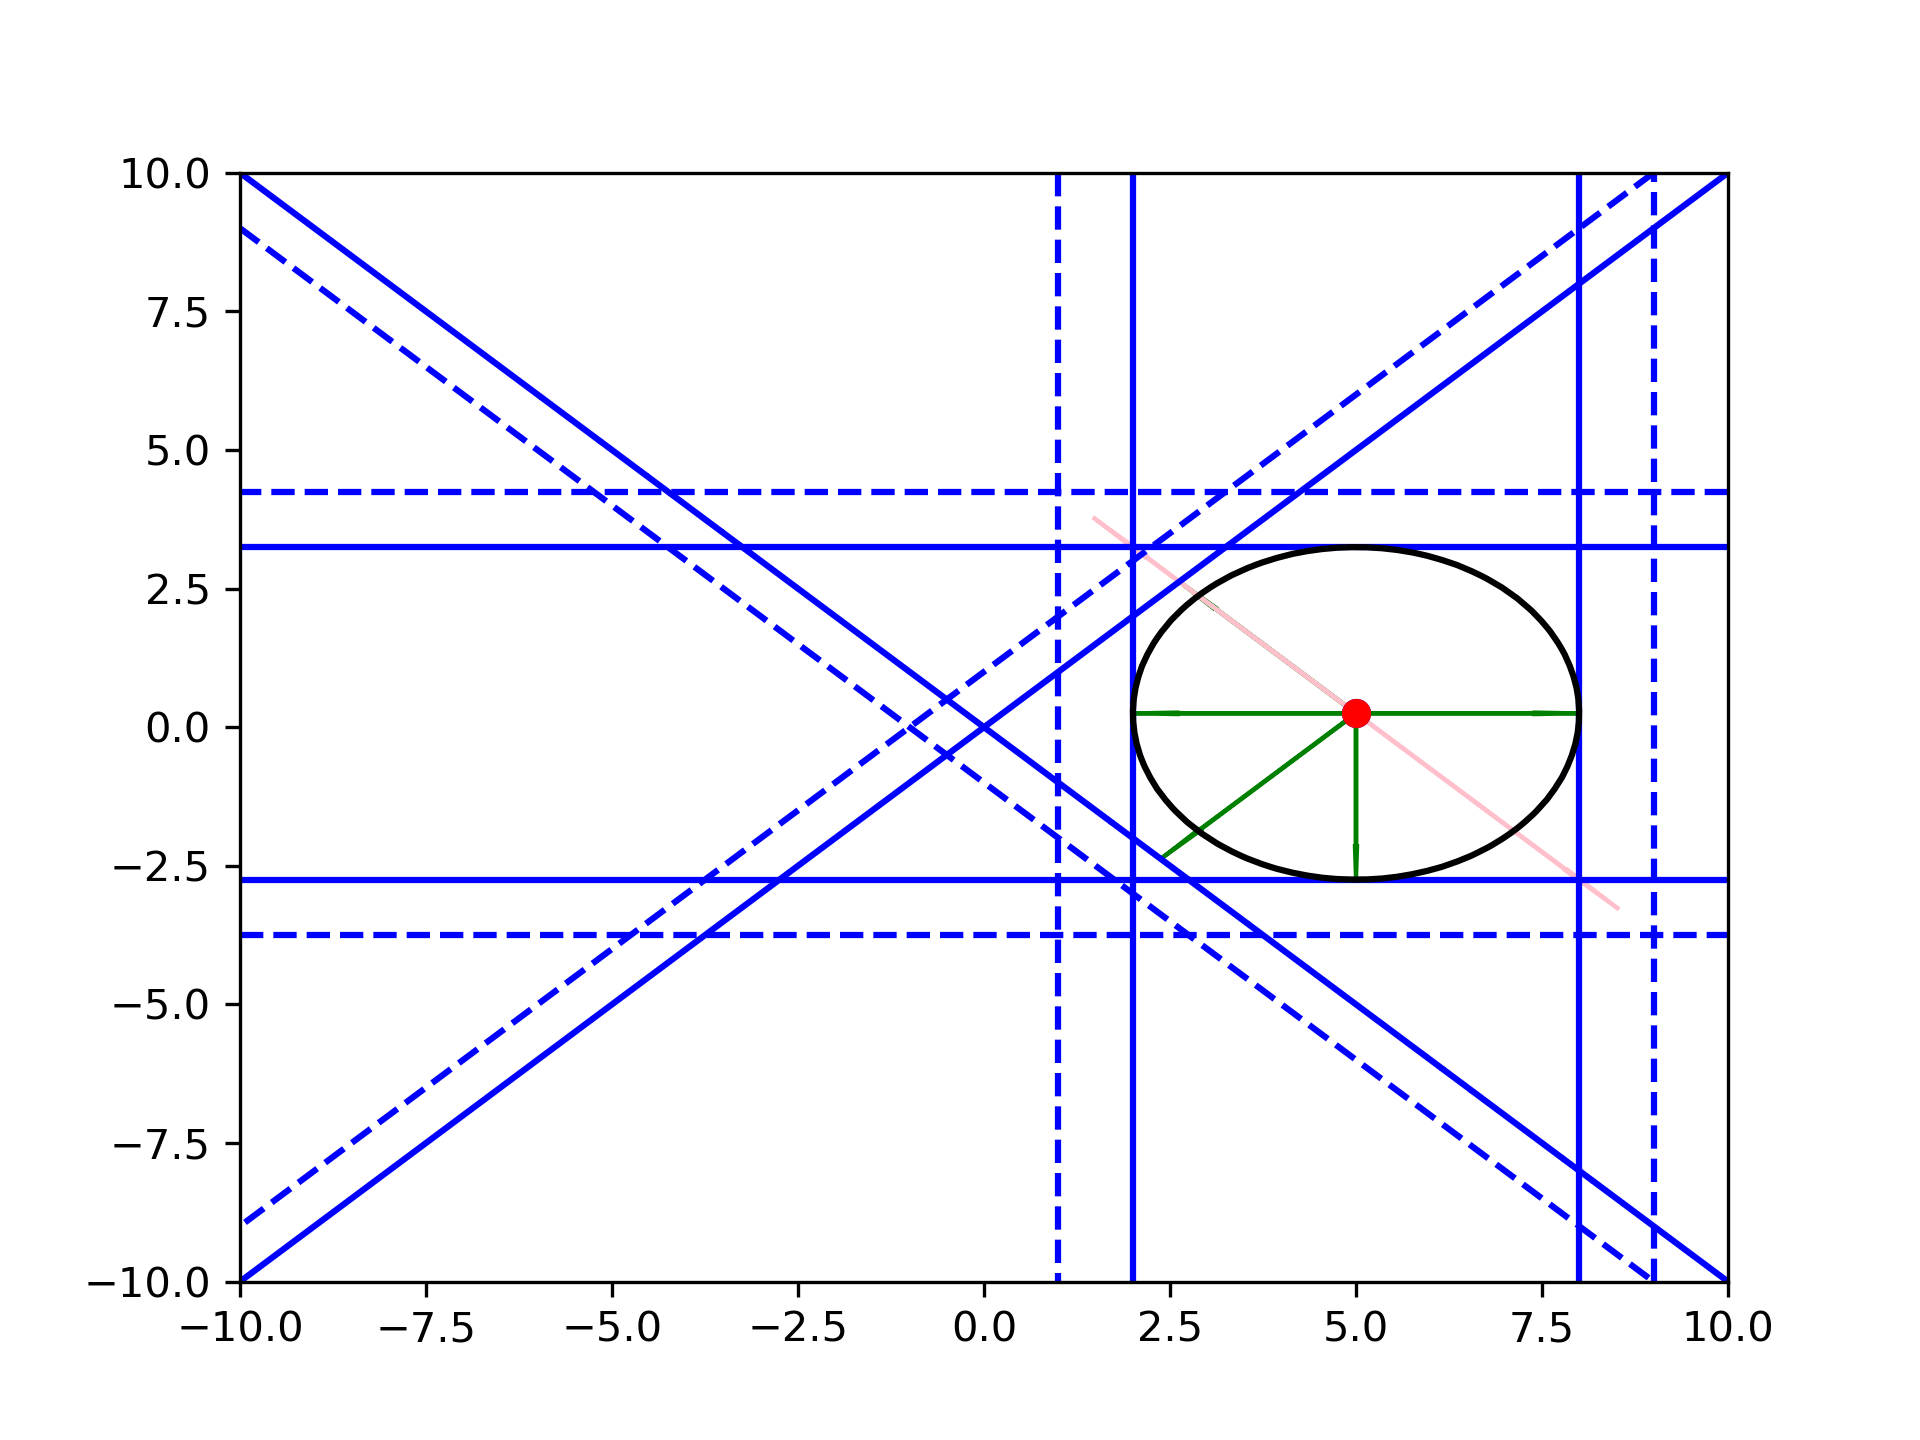
\includegraphics[scale=0.4]{advantage_of_ellipse_1.png}
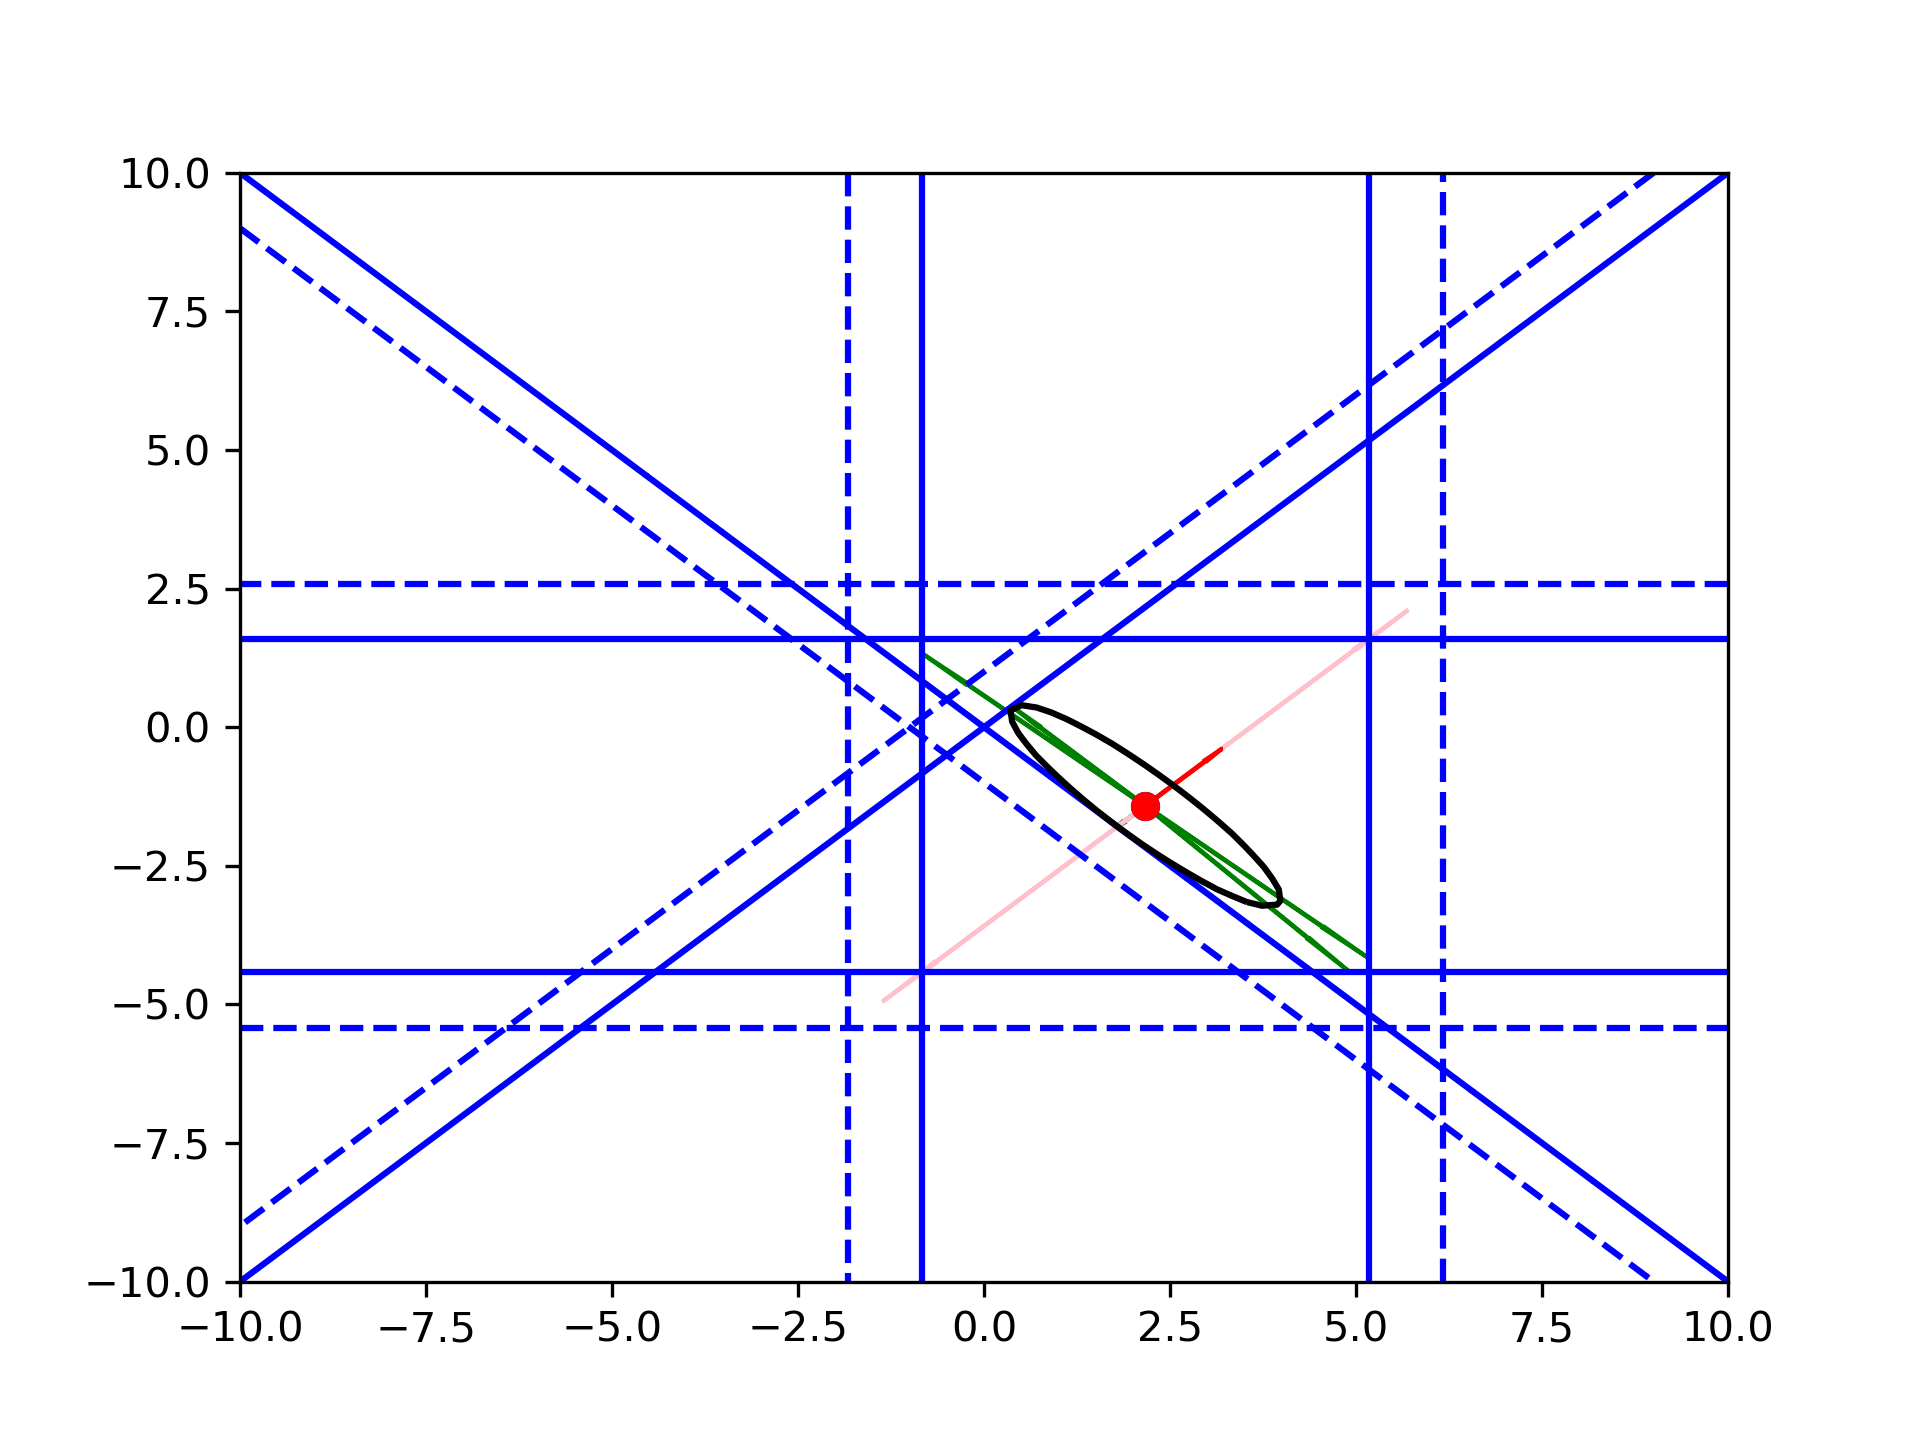
\includegraphics[scale=0.4]{advantage_of_ellipse_2.png}



\subsection{Search everything}
Another simple approach is to define the ellipse as to maximize the area within the ellipse.
That is, we add the constraints directly to the trust region subproblem.
$$\mu^k = \sup_{\mu \in \mathcal{F}^k} V(\mu))$$
This has the advantage that it captures much of the feasible region.
However, one problem with this search is that it can force the trust region away from the desired direction.

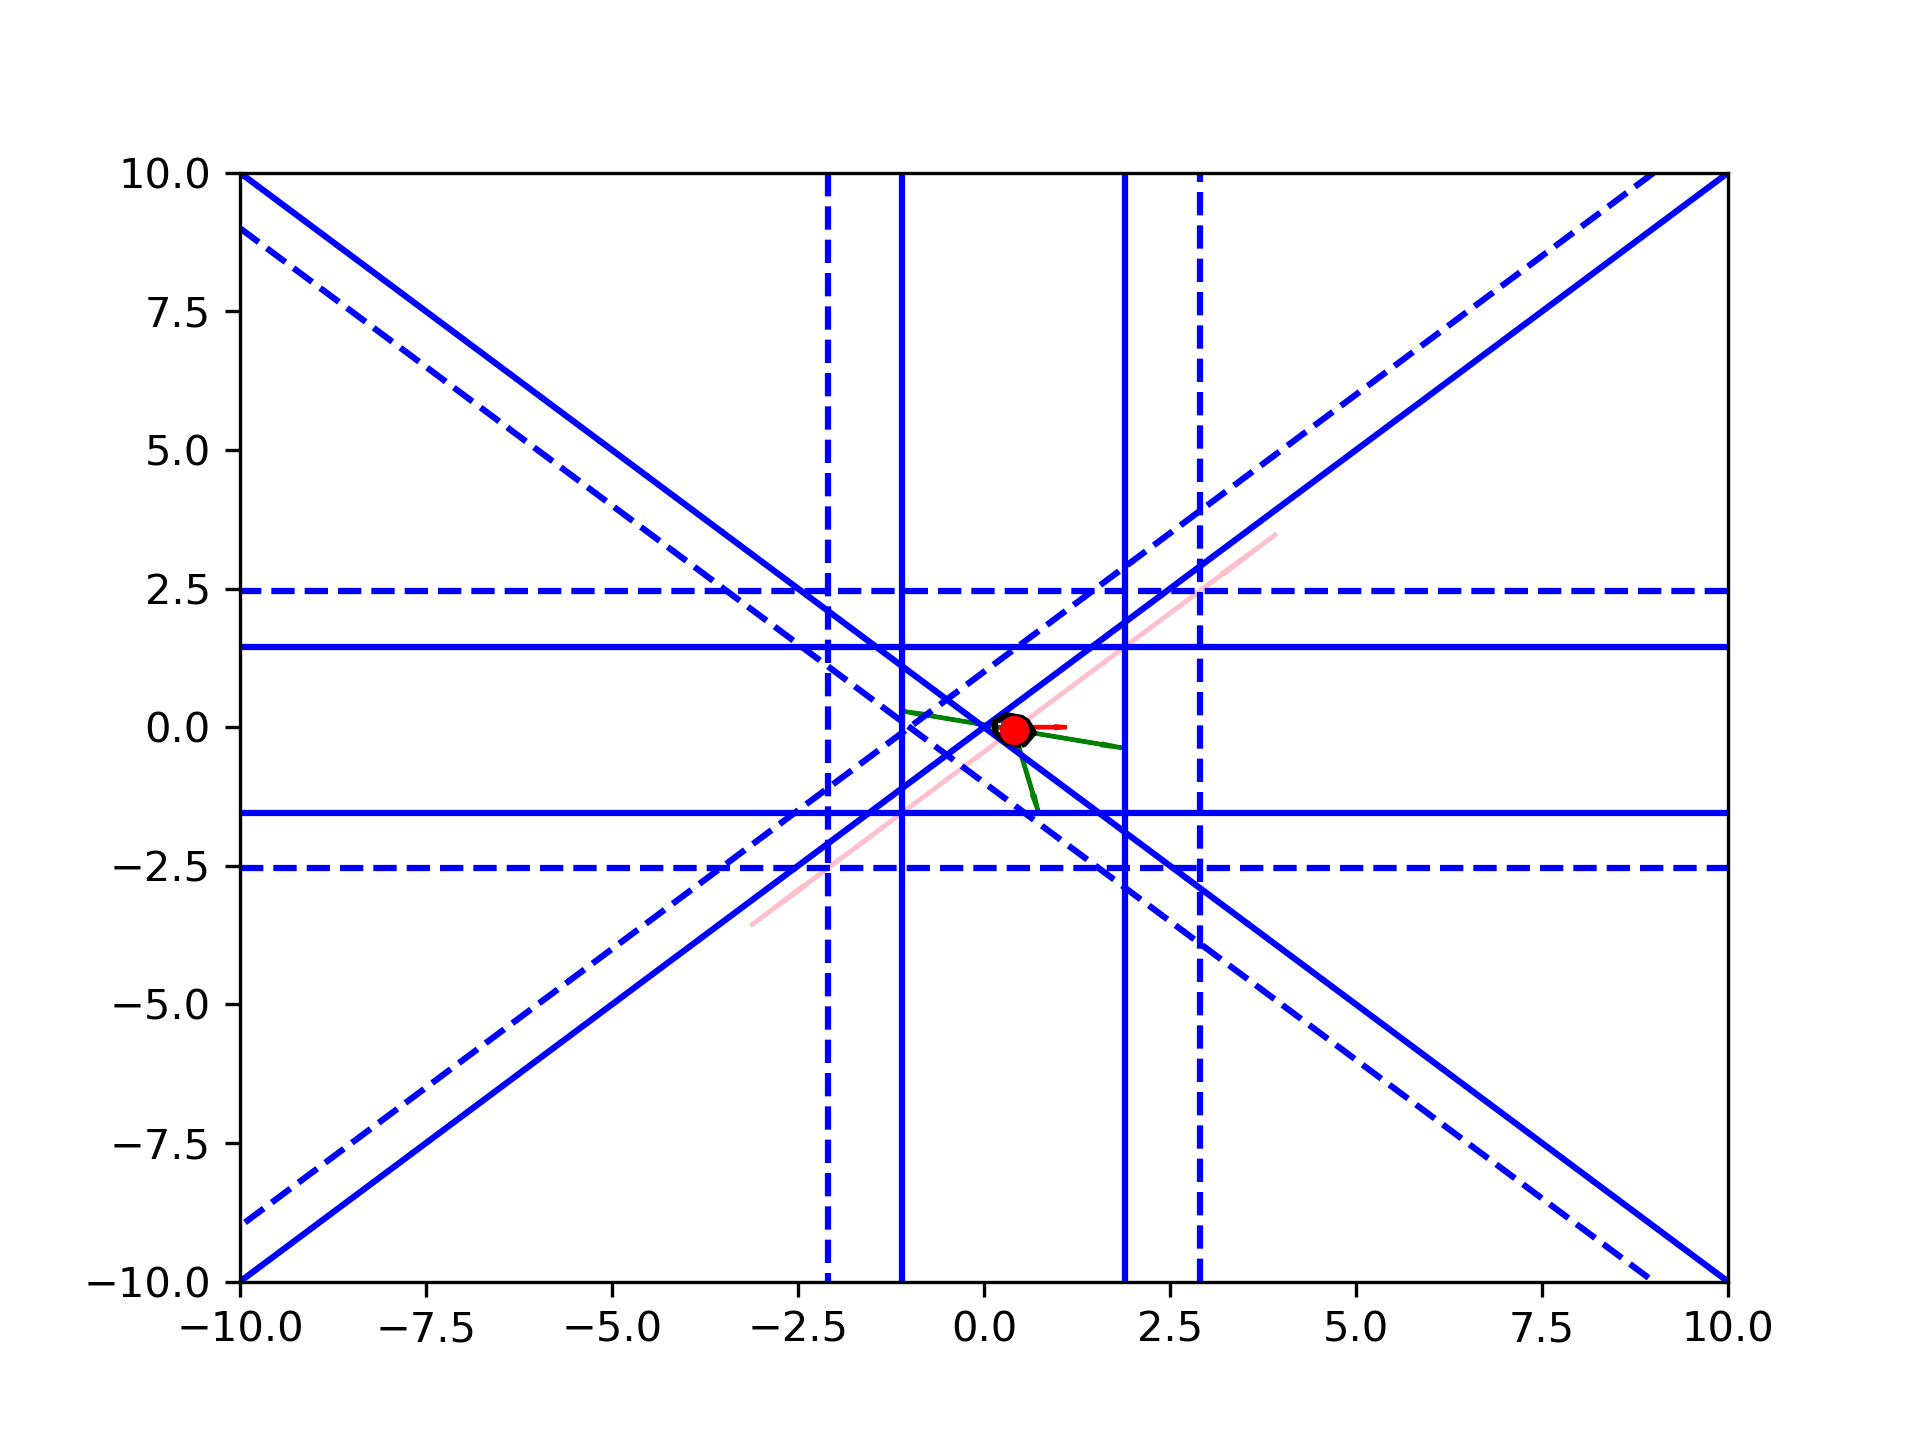
\includegraphics[scale=0.4]{everything_runs_1.png}
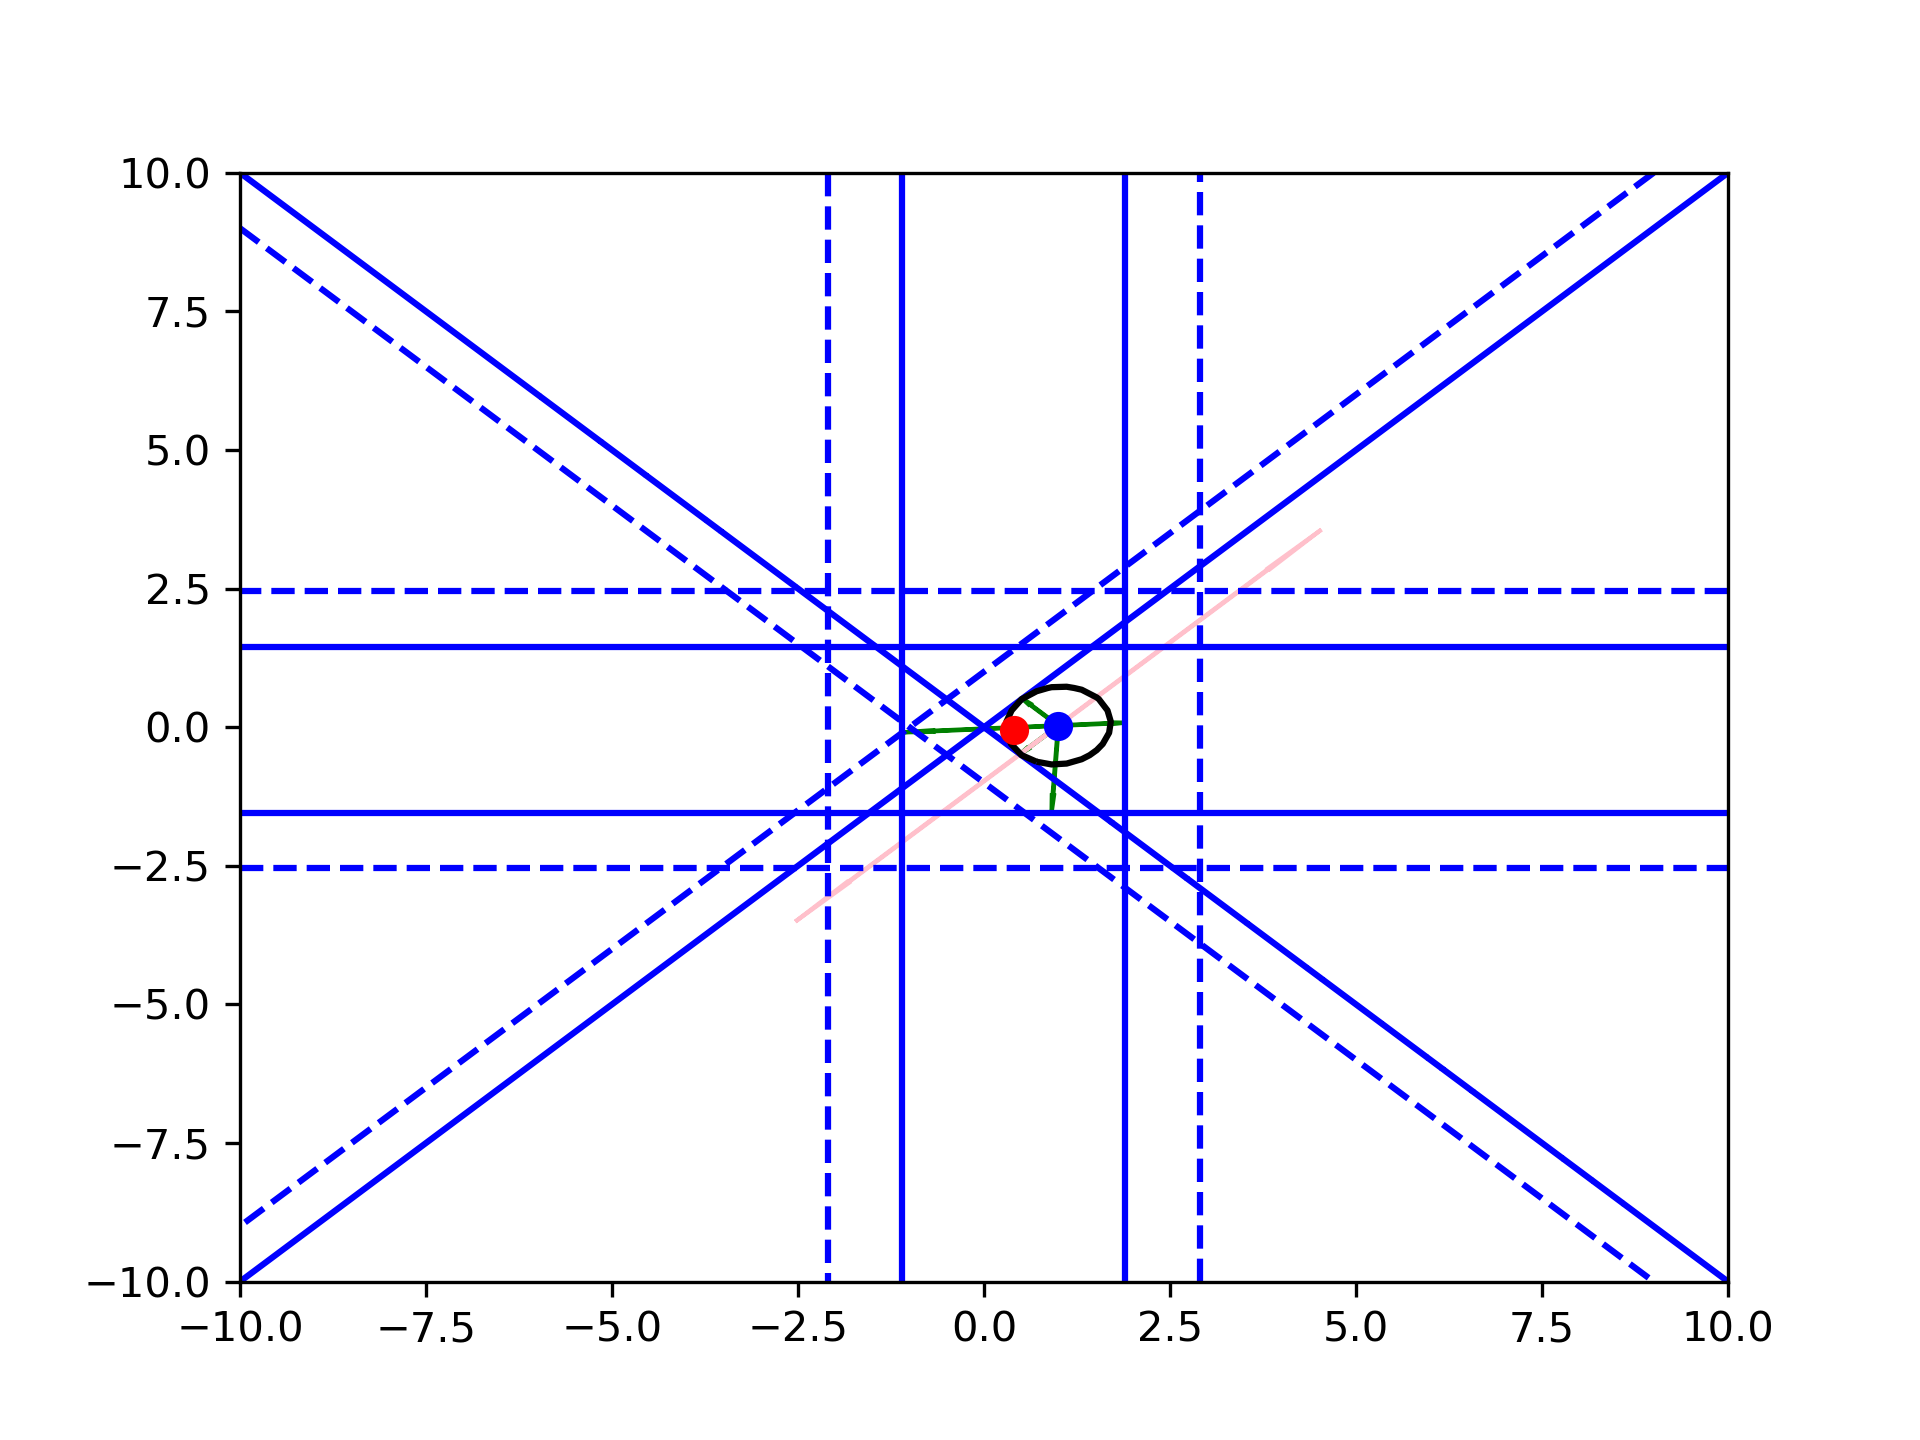
\includegraphics[scale=0.4]{everything_runs_2.png}


One attempt to fix this problem is by limiting the search direction for the center of the ellipse.

\subsection{Line searches}
Although the minimum of problem $P$ can appear anywhere within the trust region, there are some reasons for expecting it to be at a ``vertex."
If it lies on the interiorer, there is little need for using constrained approaches once near the solution.

The ellipse with maximum volume, however, tends to lead away from vertices because there is more space away from vertices.
One way of trying to leave the direction towards a vertex within the trust region, while still allowing to incease the ellipse volume is by limiting the search for the new center to lie on line segments starting at the current iterate.

For example, our first attempt was to simply search a line directed away from the closest constraint.
This has obvious problems though, as we should avoid letting the new center get closer to another constraint:

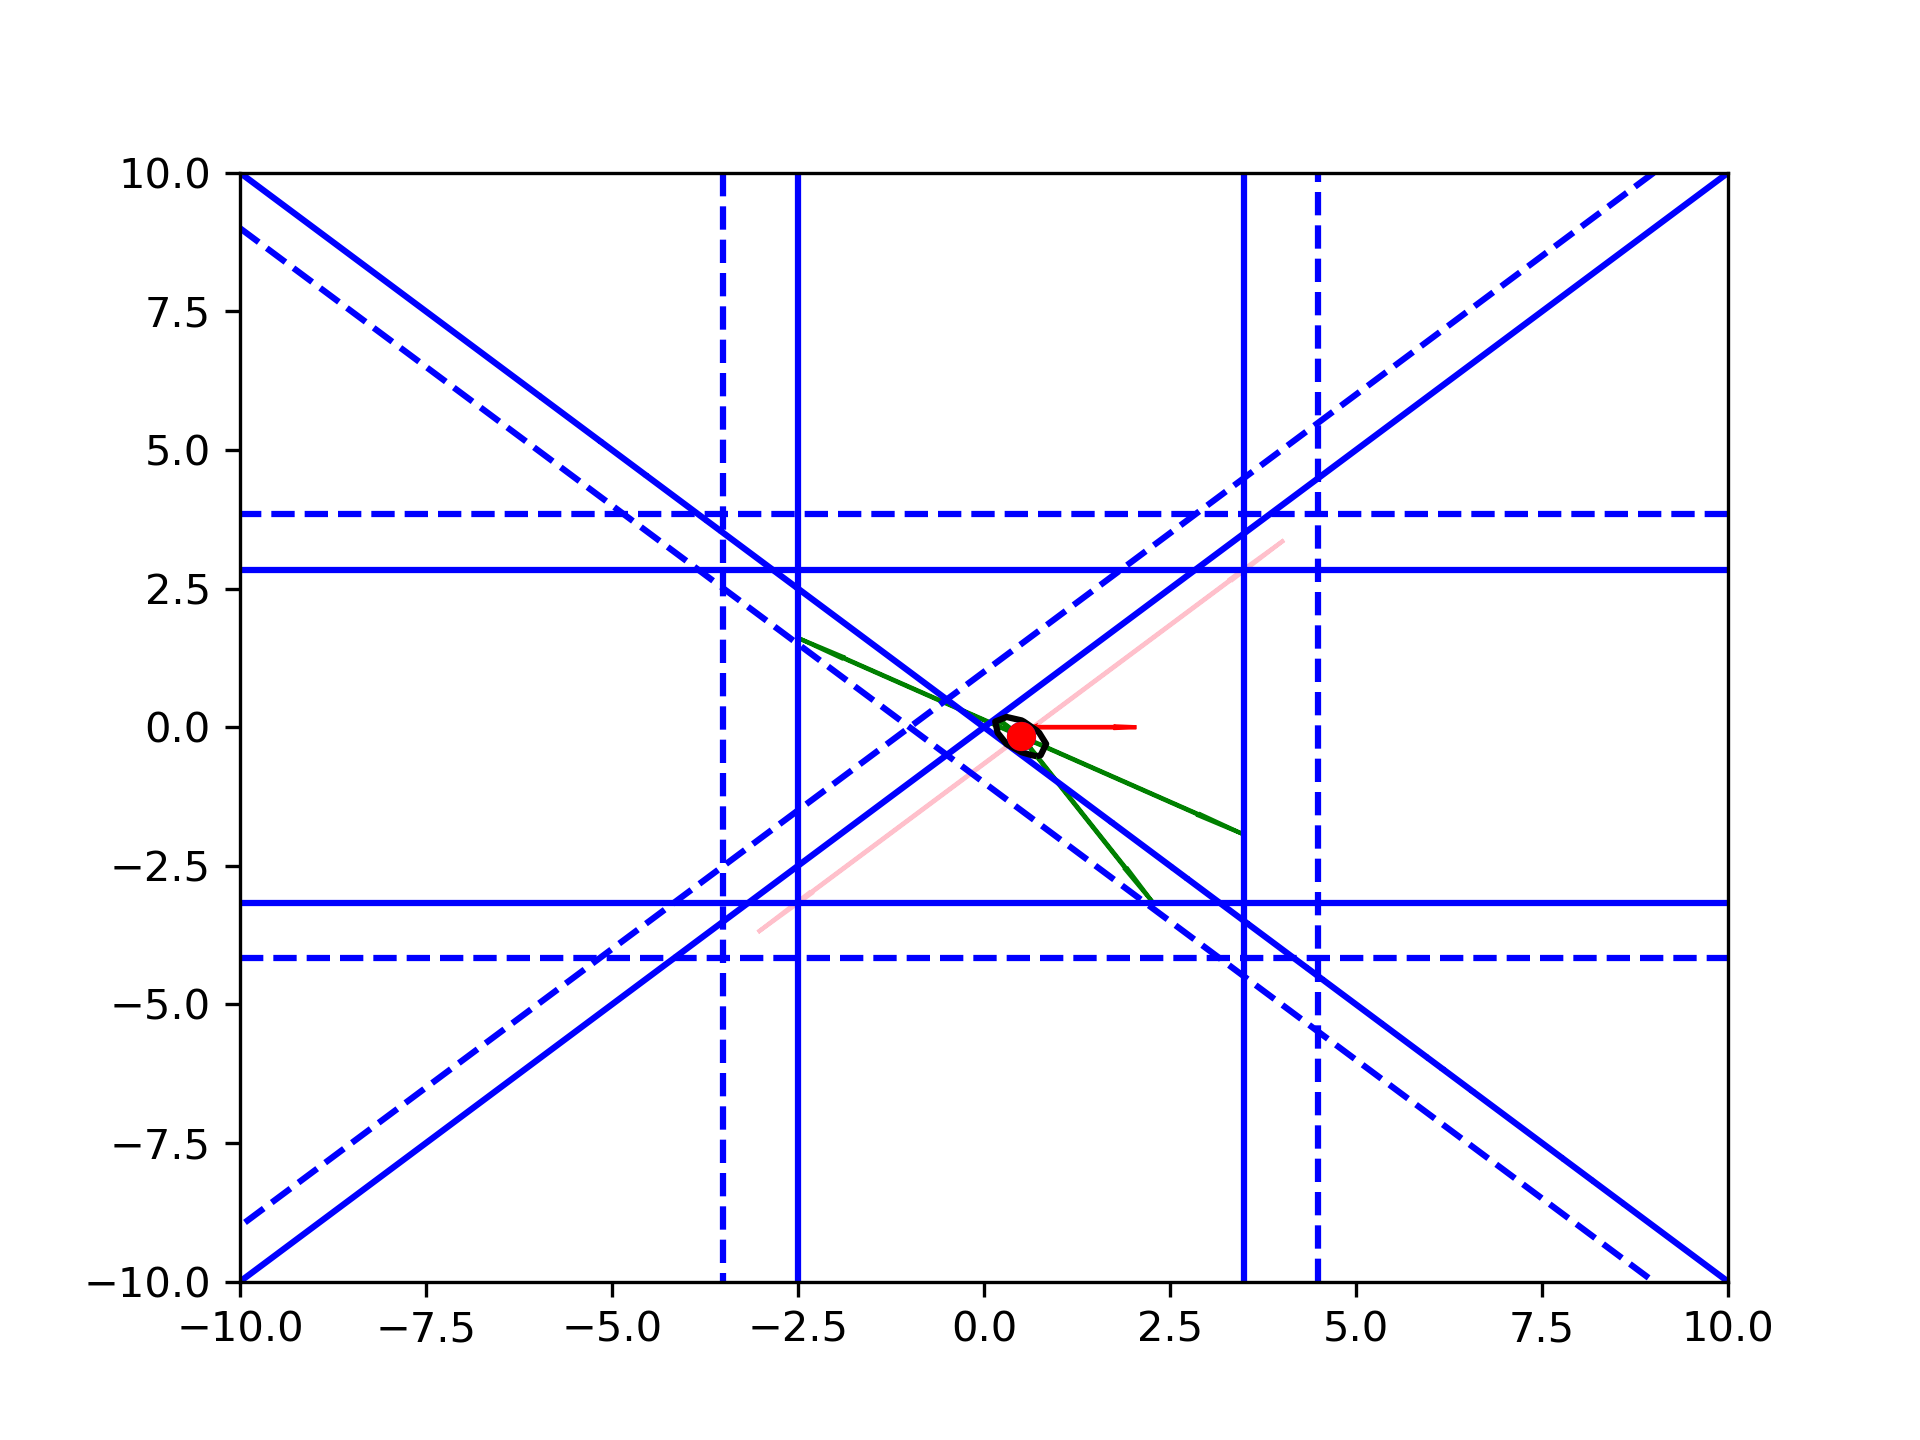
\includegraphics[scale=0.4]{line_1.png}
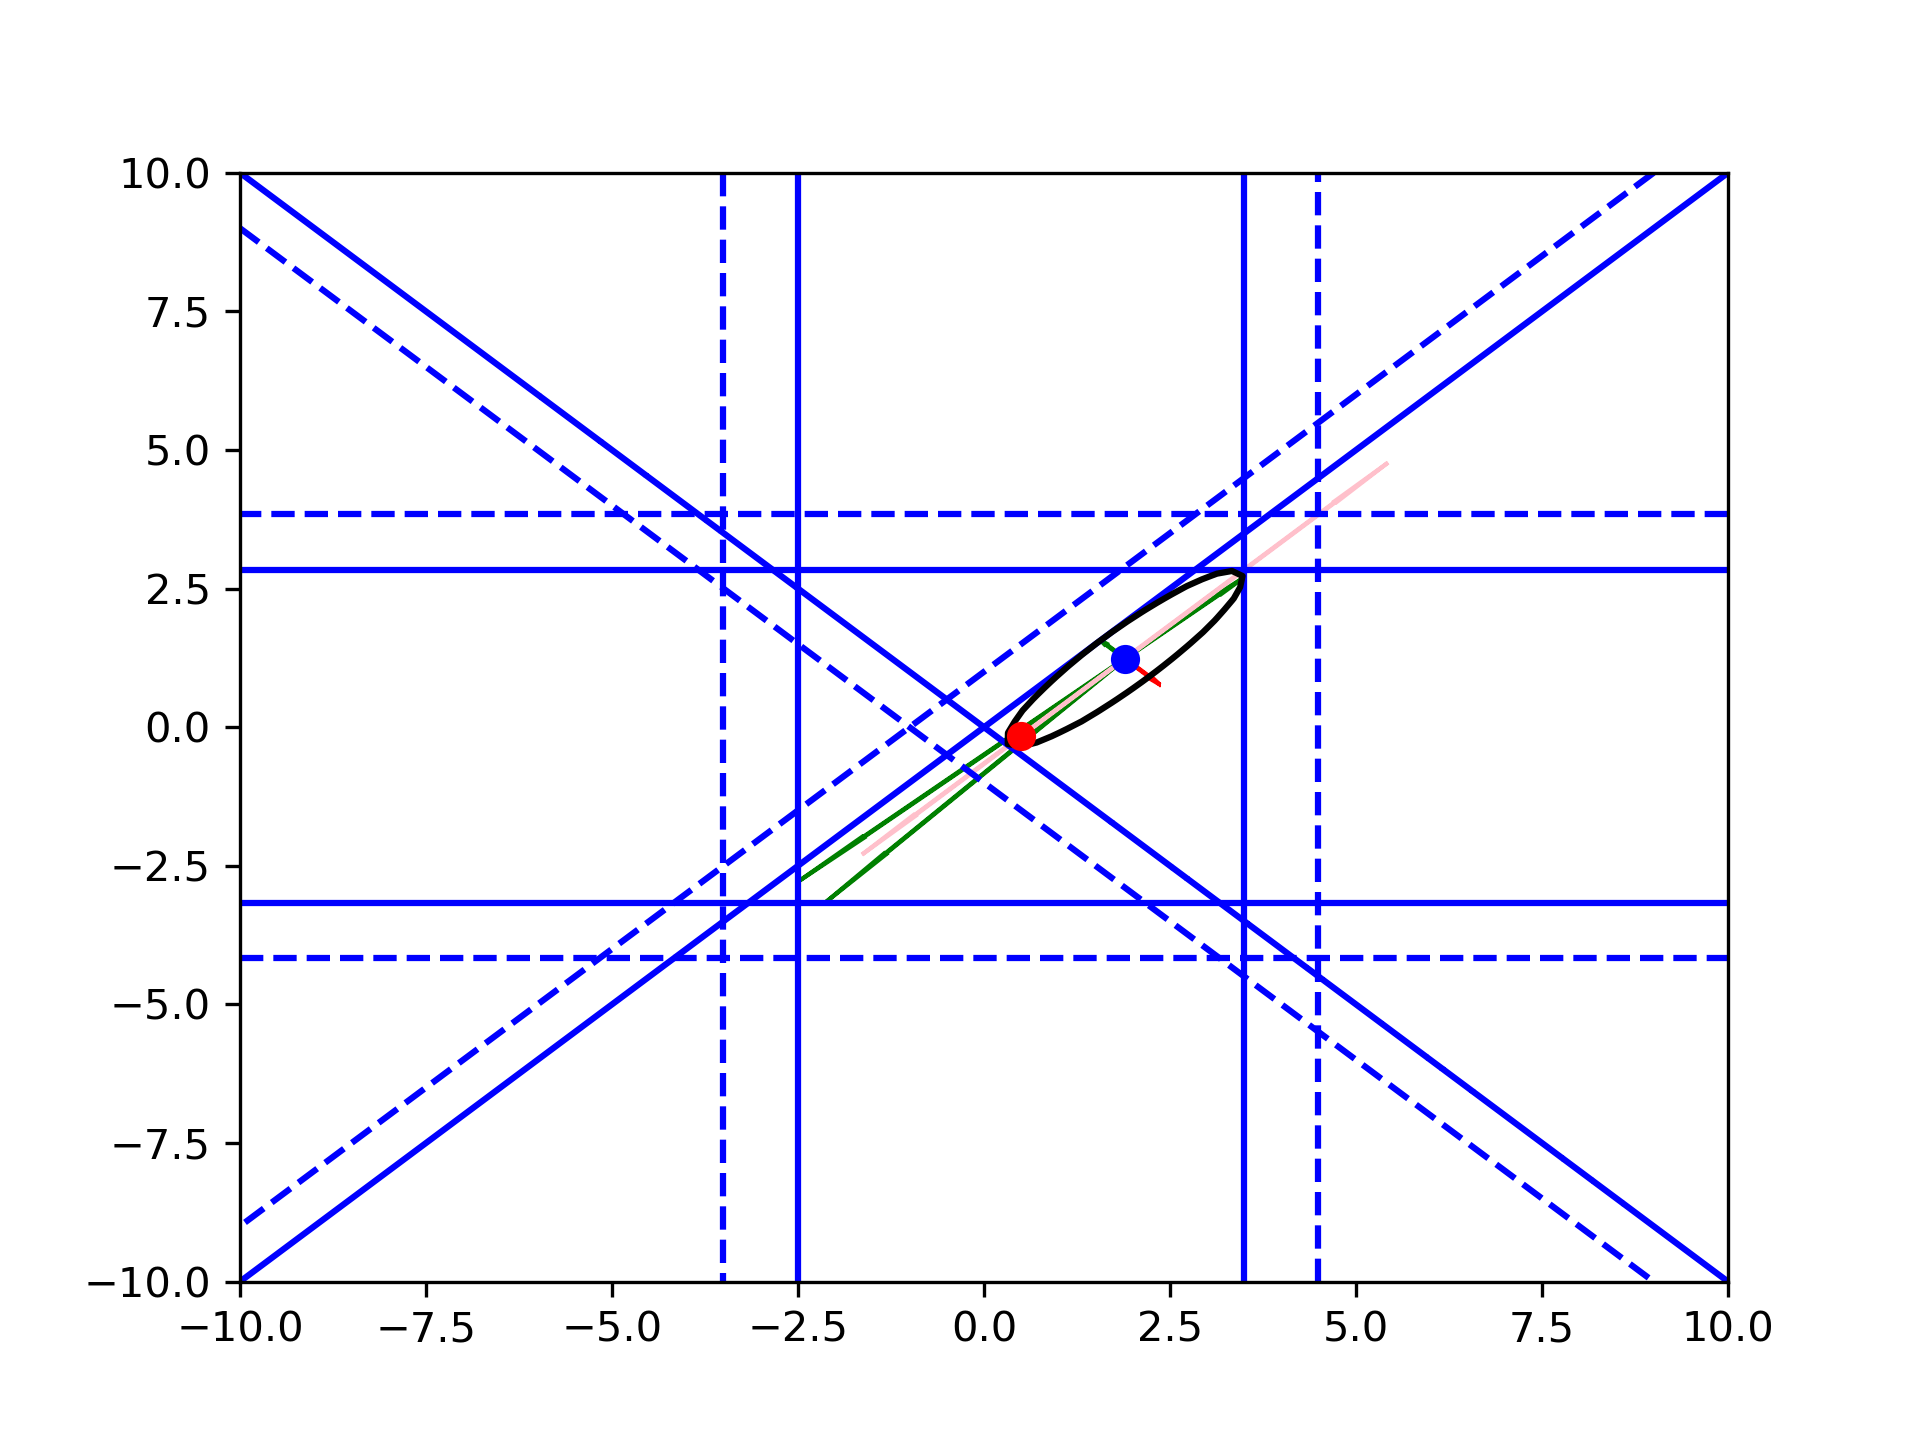
\includegraphics[scale=0.4]{line_2.png}


To fix this, we break the line into segments based on the nearest constraint.
We find the center that maximizes the volume of the ellipse after restricting it to lie on a ray perpendicular to the nearest constraint.
Nearest here means means the constraint with the smallest distance from the iterate to the projection of that iterate onto the constraint.
If there are two constraints that are both closer than all others, then we follow a ray whose points are equidistant from both of these constraints.

We search along this away from the current iterate until we reach a point that has the same distance to another constraint as the nearest to the iterate.
We could then in general continue to follow line segments by always travelling away from the nearest constraints.
However, after we include enough constraints, we will eventually once again head away from a vertex.

This means that we can define the a class of searches that each use a different number of line segments to search.
In this paper, we consider one and two line segments.

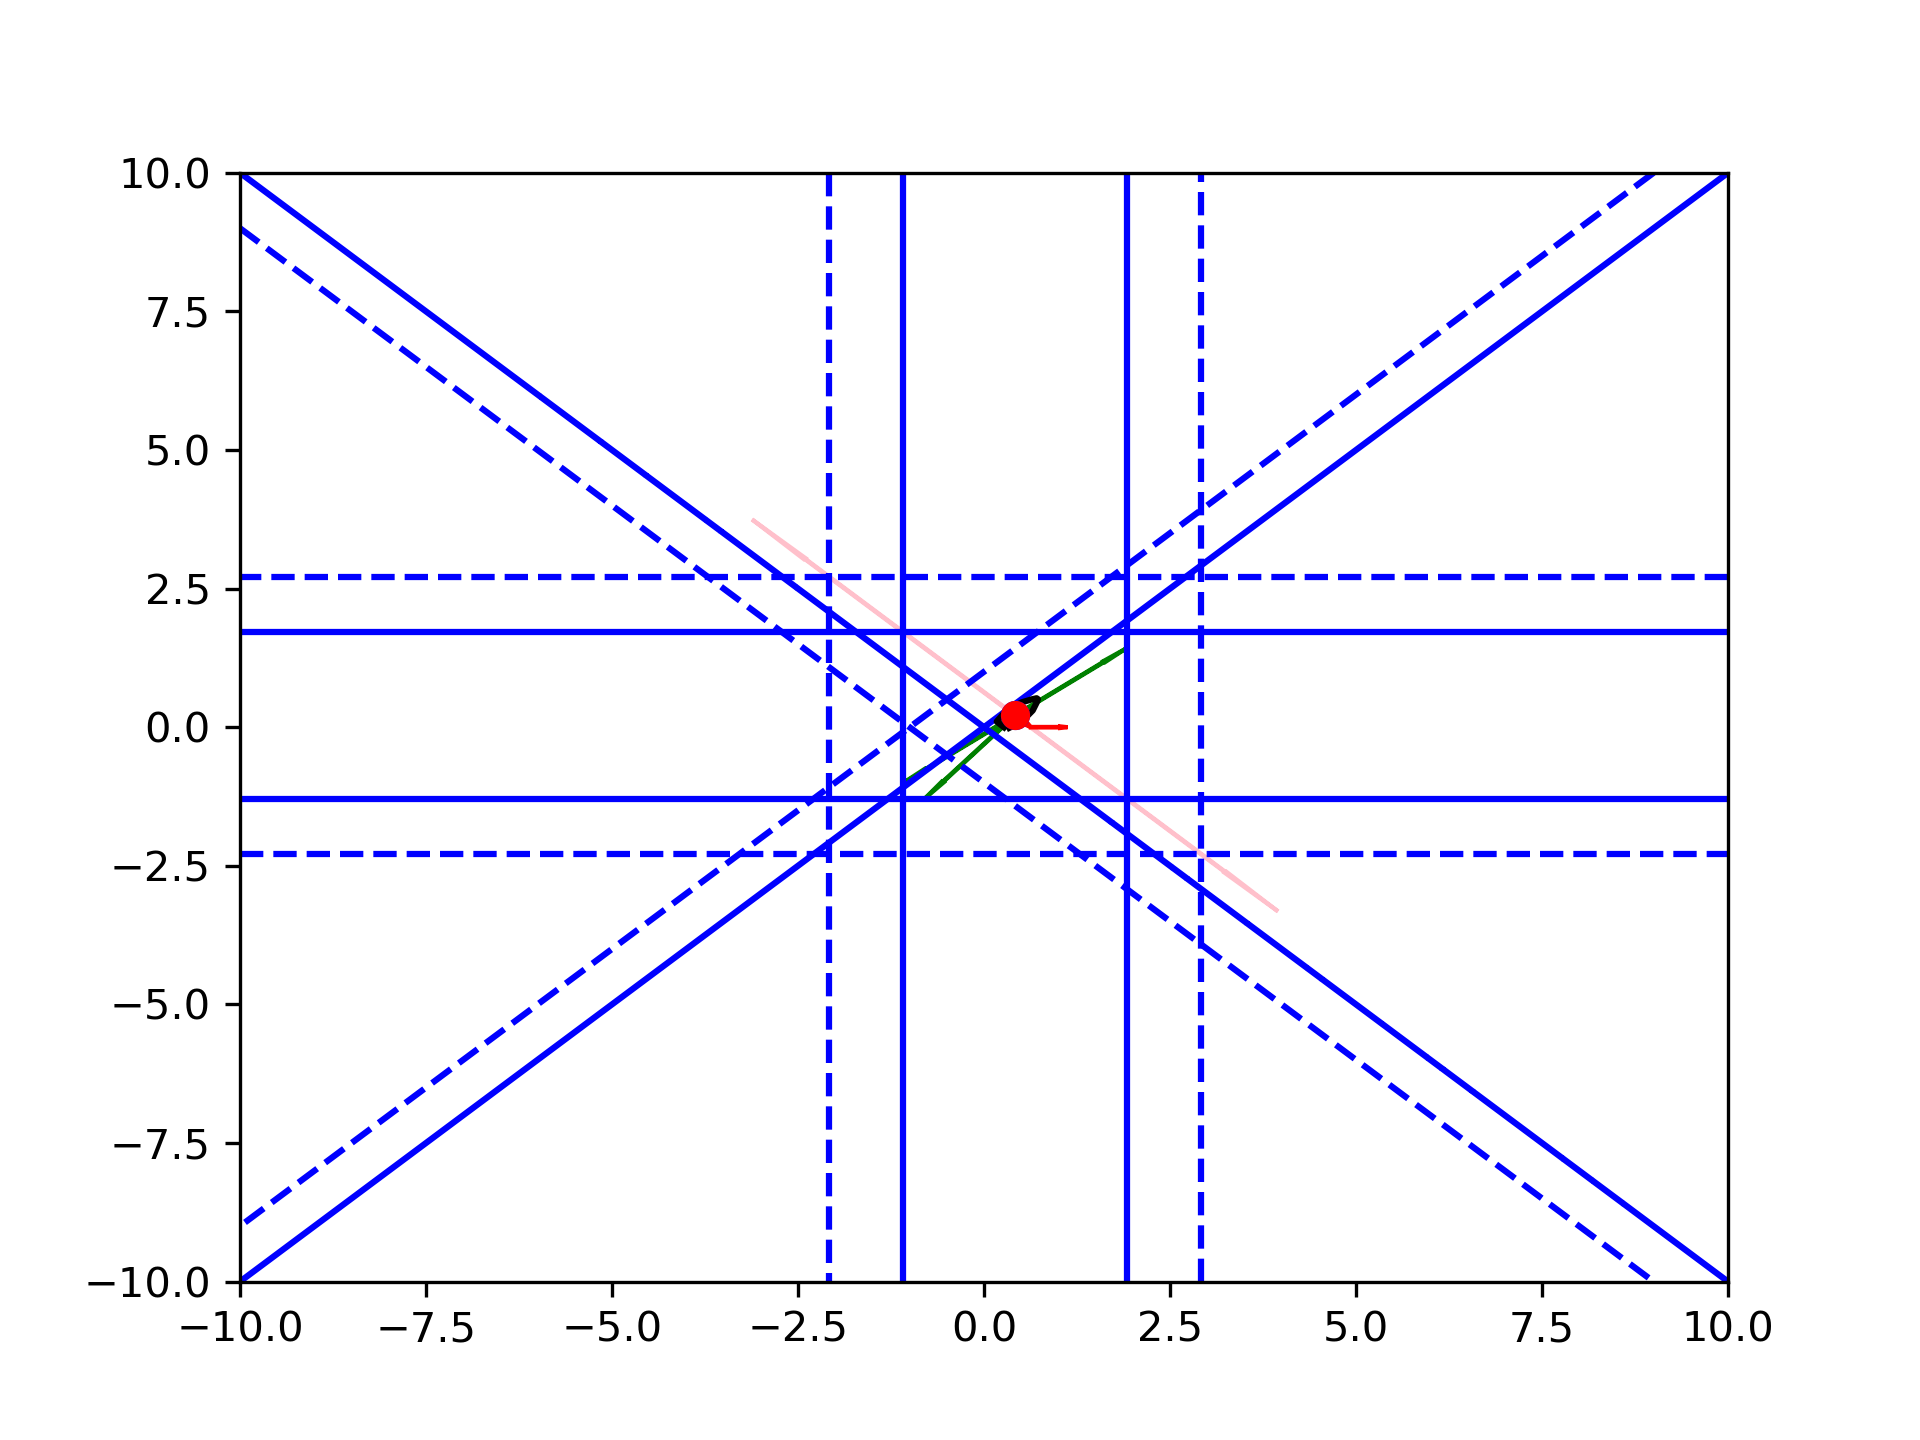
\includegraphics[scale=0.4]{run_away_1.png}
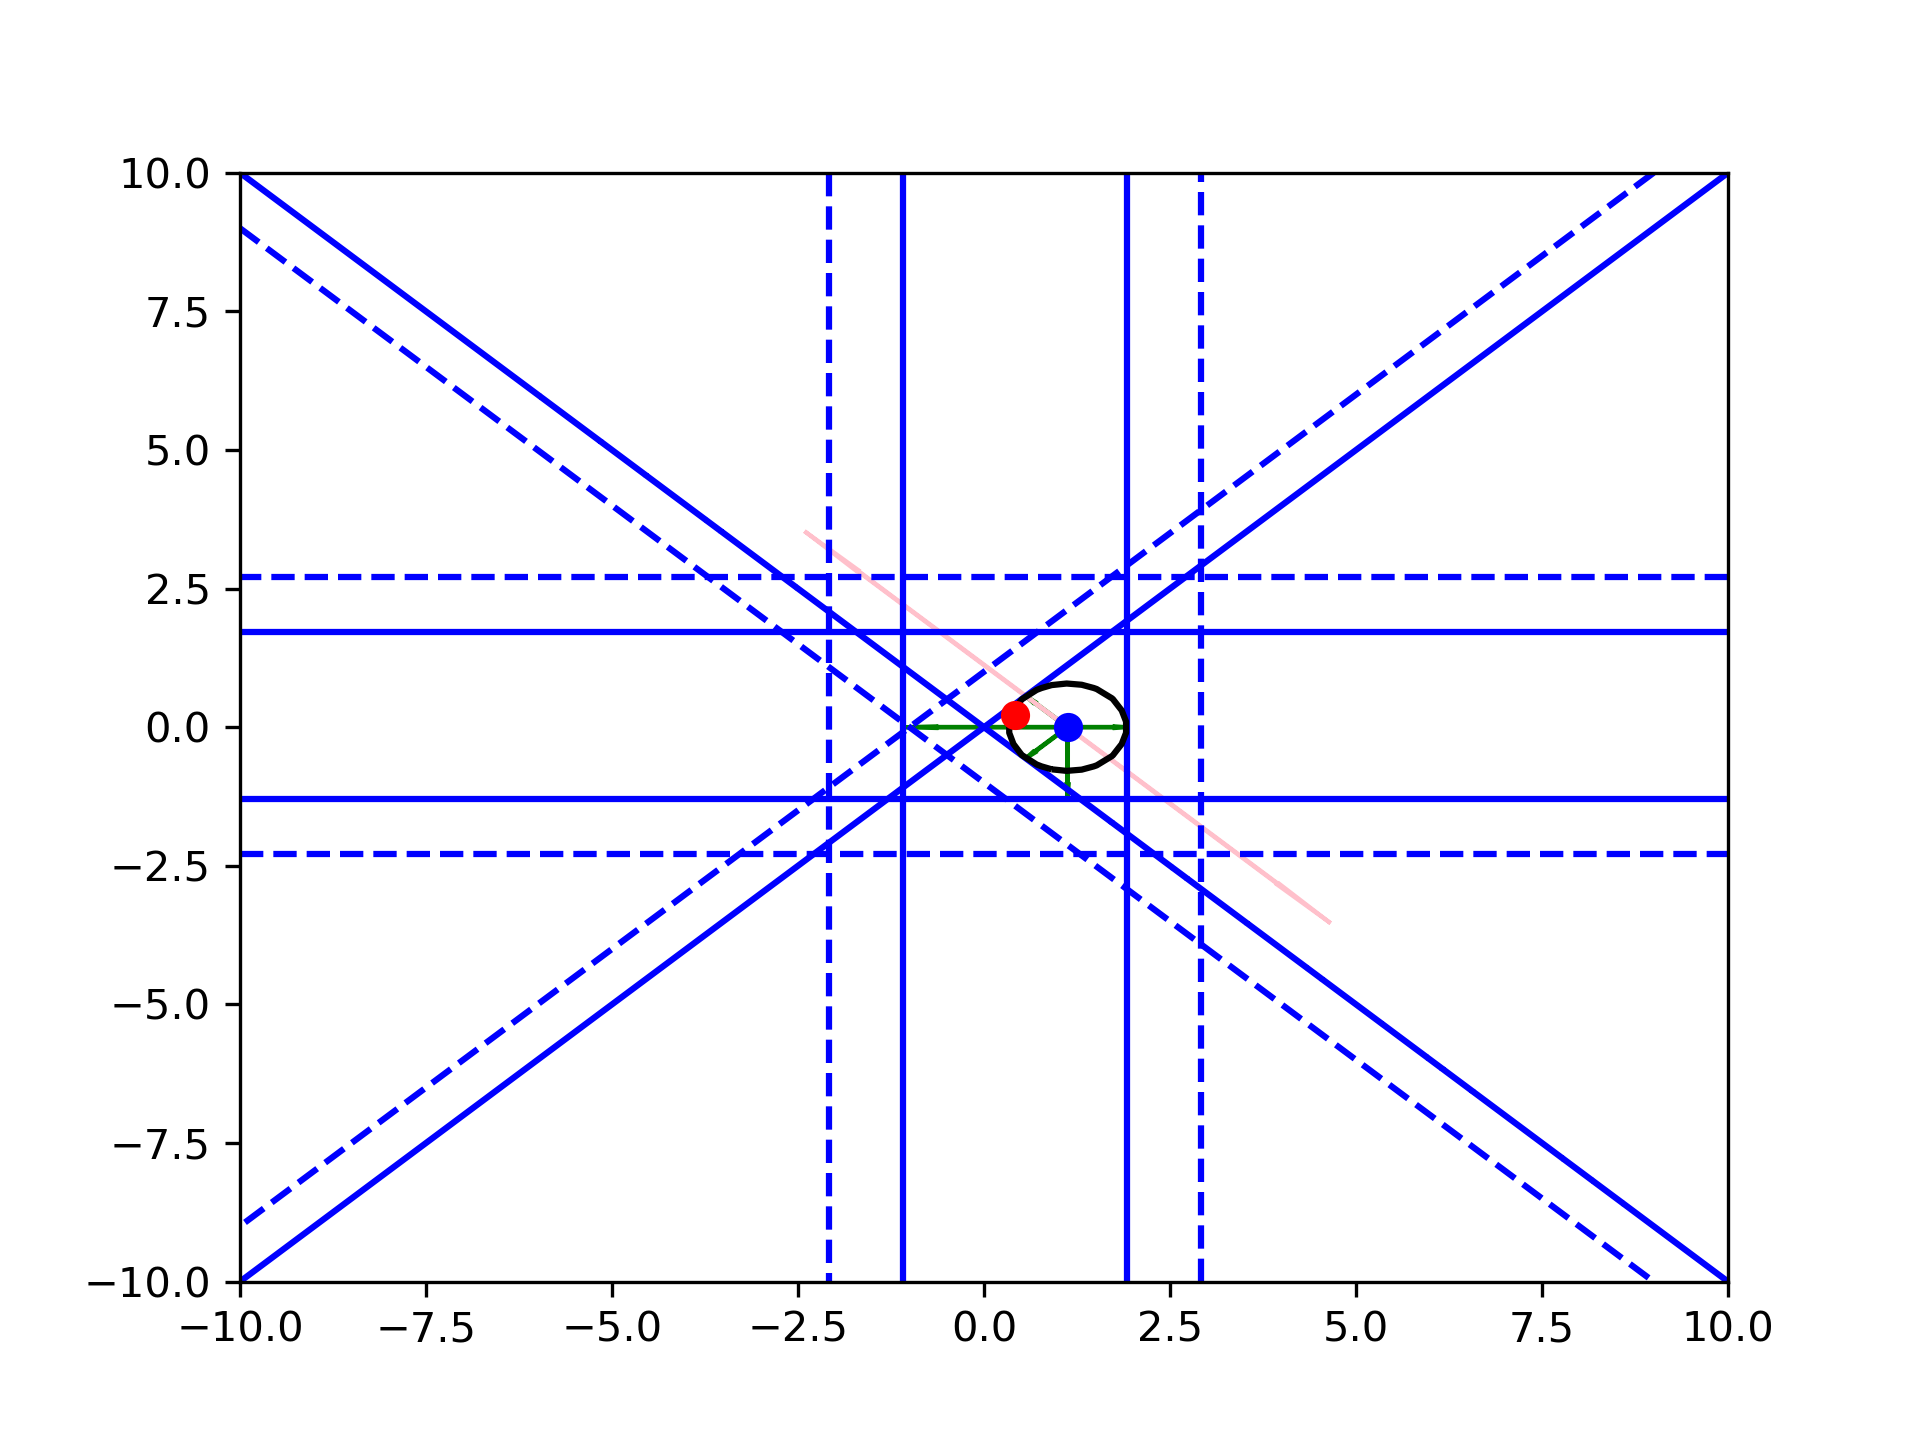
\includegraphics[scale=0.4]{run_away_2.png}

\section{Analysis Thoughts}

We plan to leverage convergence results found in \cite{Conejo:2013:GCT:2620806.2621814} which presents very general global convergence results for derivative free algorithms over convex constraints.
A key step in showing using this proof will be satisfying the efficiency condition
$m_f(x_{k}) - m_f(x_{k+1}) \ge c \chi(x_{k+1}) \min\{ \frac{\chi(x_{k+1})}{1 + \|\nabla^2m_f(x_{k+1})\|}, \Delta_k, 1 \}$.

Should $\rho$ include the constraints.

\section{Extensions}
The ellipse may be preferrable when we wish to avoid getting too close to the constraints.



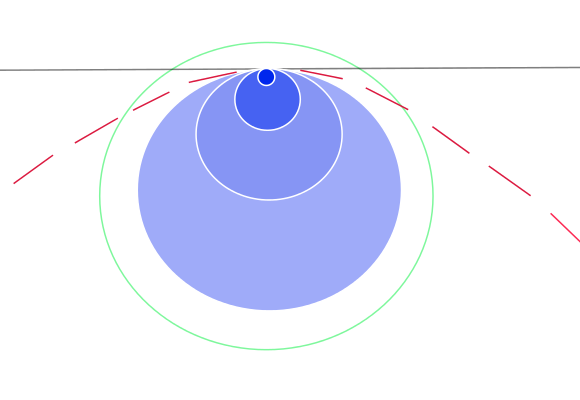
\includegraphics[width=200px]{images/second_order_critical_point.png}


\section{Results}

the example problem I have been working with
    linear constraints
%\min \alpha sin(x) + \beta (minor * x + (y - self.amplitude * x sin(freq * x)) ^ 2 
%
%		return 0.9 * (x[0]) + 0.1 * (self.minorSpeed * x[0] + (x[1] - self.amplitude * x[0] * sin(self.freq * x[0])) ** 2)





\begin{center}
\begin{tabular}{ c c c }
 Algorithm & Iterations & Evaluations \\ 
 Search everything (include the original) & 24 & 169 \\  
 Search everything & 19 & 106    \\
 One line segment & 21 & 86 \\
 Two line segments & 23 & 115 \\
 Circle search everywhere &  & 133 \\
\end{tabular}
\end{center}

\newpage

\newpage

\bibliography{bibliography}
\bibliographystyle{ieeetr}

\end{document}


